\documentclass[10pt]{article}
\renewcommand{\baselinestretch}{1.8}

\usepackage[letterpaper, margin=1in]{geometry}
\usepackage{tikz-qtree}
\usepackage{algorithm}
\usepackage{algpseudocode}
\makeatletter
\renewcommand{\ALG@beginalgorithmic}{\footnotesize}
\makeatother
\usepackage{graphicx}
\usepackage{subcaption}
%\usepackage{showkeys}
\usepackage{amsmath}


\usepackage{multicol}
\setlength\columnsep{24pt}

\algnewcommand\algorithmicforeach{\bf{for each}}
\algdef{S}[FOR]{ForEach}[1]{\algorithmicforeach\ #1\ \algorithmicdo}

\algdef{S}[FUNCTION]{Function}
   [3]{{\tt{\sl{#1}}} {\tt{#2}}\ifthenelse{\equal{#3}{}}{}{\tt{(#3)}}}
  
\algdef{E}[FUNCTION]{EndFunction}
   [1]{\algorithmicend\ \tt{{#1}}}

\algrenewcommand\Call[2]{\tt{{#1}\ifthenelse{\equal{#2}{}}{}{(#2)}}}
   
\newcommand\keywordfont{\sffamily\bfseries}
\algrenewcommand\algorithmicend{{\keywordfont end}}
\algrenewcommand\algorithmicfor{{\keywordfont for}}
\algrenewcommand\algorithmicforeach{{\keywordfont for each}}
\algrenewcommand\algorithmicdo{{\keywordfont do}}
\algrenewcommand\algorithmicuntil{{\keywordfont until}}
\algrenewcommand\algorithmicfunction{{\keywordfont function}}
\algrenewcommand\algorithmicif{{\keywordfont if}}
\algrenewcommand\algorithmicthen{{\keywordfont then}}
\algrenewcommand\algorithmicelse{{\keywordfont else}}
\algrenewcommand\algorithmicreturn{{\keywordfont return}}

\renewcommand\thealgorithm{}
\newcommand{\setalglineno}[1]{%
  \setcounter{ALC@line}{\numexpr#1-1}}

\newcommand{\sub}[1]{\textsubscript{#1}}
\renewcommand{\tt}[1]{\texttt{#1}}
\renewcommand{\sl}[1]{\textsl{#1}}
\renewcommand{\it}[1]{\textit{#1}}
\renewcommand{\sc}[1]{\textsc{#1}}
\renewcommand{\bf}[1]{\textbf{#1}}
\newcommand{\nf}[1]{{\normalfont{\texttt{#1}}}}
\newcommand{\cmt}[1]{\Comment{#1}}
\newcommand{\head}{head}
\newcommand{\size}{size }

\usepackage{amsmath,amssymb,amsthm}
\newtheorem{theorem}{Theorem}
\newtheorem{lemma}[theorem]{Lemma}
\newtheorem{corollary}[theorem]{Corollary}
\newtheorem{observation}[theorem]{Observation}
\theoremstyle{definition}
\newtheorem{definition}[theorem]{Definition}
\newtheorem{invariant}[theorem]{Invariant}


\begin{document}
\title{Wait-free Queues with Polylogarithmic Step Complexity}
\author{Hossein Naderibeni \\supervised by Eric Ruppert}
\maketitle

\begin{abstract}
In this work, we are going to introduce a novel lock-free queue implementation.
Linearizability and lock-freedom are standard requirements for designing shared data structures. All existing linearizable, lock-free queues in the literature have a common problem in their worst case called CAS Retry Problem. Our contribution is solving this problem while outperforming the previous algorithms.
\end{abstract}

\tableofcontents
\pagebreak
\section{Introduction}
Shared data structures have become an essential field in distributed algorithms research.
We are reaching the physical limits of how many transistors we can place on a CPU core. The industry solution to provide more computational power is to increase the number of cores of the CPU. This is why distributed algorithms have become important. It is not hard to see why multiple processes cannot update sequential data structures designed for one process. For example, consider two processes trying to insert some values into a sequential linked list simultaneously. Processes $p,q$ read the same tail node, $p$ changes the next pointer of the tail node to its new node and after that $q$ does the same. In this run, $p$'s update is overwritten. One solution is to use locks; whenever a process wants to do an update or query on a data structure, the process locks it, and others cannot use it until the lock is released. Using locks has some disadvantages; for example, one process might be slow, and holding a lock for a long time prevents other processes from progressing. Moreover, locks do not allow complete parallelism since only the one process holding the lock can make progress. 


The question that may arise is, ``What properties matter for a lock-free data structure?'', since executions on a shared data structure are different from sequential ones, the correctness conditions also differ. To prove a concurrent object works perfectly, we have to show it satisfies safety and progress conditions. A \textit{safety condition} tells us that the data structure does not return wrong responses, and a \textit{progress property} requires that operations eventually terminate.


The standard safety condition is called \textit{linearizability}, which ensures that for any concurrent execution on a linearizable object, each operation should appear to take effect instantaneously at some moment between its invocation and response. Figure \ref{fig::goodexample} is an example of an execution on a linearizable  queue that is initially empty. The arrow shows time, and each rectangle shows the time between the invocation and the termination of an operation. Since \texttt{Enqueue(A)} and \texttt{Enqueue(B)} are concurrent, \texttt{Enqueue(B)} may or may not take effect before \texttt{Enqueue(A)}. The execution in Figure \ref{fig::badexample} is not linearizable since \texttt{A} has been enqueued before \texttt{B}, so it has to be dequeued first.

\begin{figure}[hbt]
  \center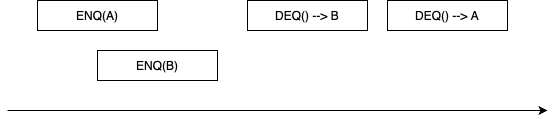
\includegraphics[scale=0.5]{pics/good}
  \caption{\label{fig::goodexample}An example of a linearizable execution. Either \texttt{Enqueue(A)} or \texttt{Enqueue(B)} could take effect first since they are concurrent.}
\end{figure}

\begin{figure}[hbt]
  \center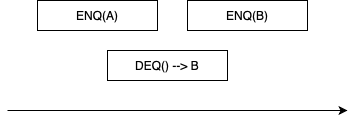
\includegraphics[scale=0.5]{pics/bad}
  \caption{\label{fig::badexample}An example of an execution that is not linearizable. Since \texttt{Enqueue(A)} has completed before \texttt{Enqueue(B)} is invoked the \texttt{Dequeue()} should return \texttt{A} or nothing.}
\end{figure}


There are various progress properties; the strongest is wait-freedom, and the more common is lock-freedom. An algorithm is \textit{wait-free} if each operation terminates after a finite number of its own steps. We call an algorithm \textit{lock-free} if, after a sufficient number of steps, one operation terminates. A wait-free algorithm is also lock-free but not vice versa; in an infinite run of a lock-free algorithm there might be an operation that takes infinitely many steps but never terminates.

In section 2 we talk about previous queues and their common problems. We also talk about polylogarithmic construction of shared objects.

Jayanti~\cite{DBLP:conf/podc/Jayanti98a} proved an $\Omega(\log p)$ lower bound on the worst-case shared-access time complexity of $p$-process universal constructions. He also introduced~\cite{DBLP:conf/podc/ChandraJT98} a construction that achieves $\textsc{O}(\log^2 p)$ shared accesses. Here, we first introduce a universal construction using $\textsc{O}(\log p)$ CAS operations~\cite{DBLP:conf/fsttcs/JayantiP05}. In section 3 we introduce a polylogarithmic step wait-free universal construction. Our main ideas in of the universal construction also appear in our Queue Algorithm (\ref{algQ}). The main short come of our universal construction is using big CAS objects. We use the universal construction as a stepping stone towards our queue algorithm, so we will not explain it in too much detail.

In section 4 we introduce a concurrent wait-free datastructure, to agree on the order of the operations invoked on some processes.

In section 5 we introduce our main work, the queue; prove its linearizability and wait-freeness.

\pagebreak
\section{Related Work}
\subsection{List-based Queues}
In the following paragraphs, we look at previous lock-free queues.
Michael and Scott~\cite{DBLP:conf/podc/MichaelS96} introduced a lock-free queue which we refer to as the MS-queue. A version of it is included in the standard Java Concurrency Package. Their idea is to store the queue elements in a singly-linked list (see Figure~\ref{fig::msq}). Head points to the first node in the linked list that has not been dequeued, and Tail points to the last element in the queue. To insert a node into the linked list, they use atomic primitive operations like \texttt{LL/SC} or \texttt{CAS}. If $p$ processes try to enqueue simultaneously, only one can succeed, and the others have to retry. This makes the amortized number of steps to be $\Omega(p)$ per enqueue. Similarly, dequeue can take $\Omega(p)$ steps.

\begin{figure}[hbt]
  \center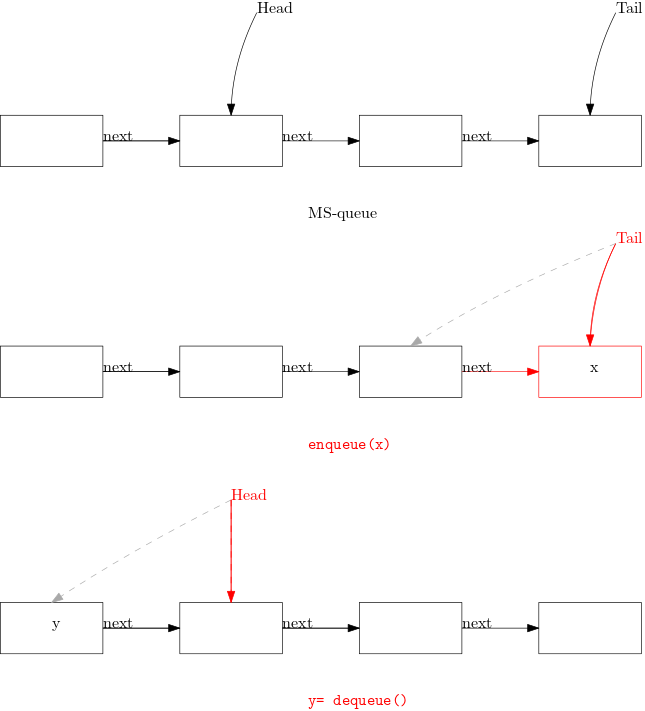
\includegraphics[scale=0.4]{pics/msqueue}
  \caption{\label{fig::msq}MS-queue structure, enqueue and dequeue operations. In the first diagram the first element has been dequeued. Red arrows show new pointers and gray dashed arrows show the old pointers.}
\end{figure}


Moir, Nussbaum, and Shalev~\cite{DBLP:conf/spaa/MoirNSS05} presented a more sophisticated queue by using the elimination technique. The elimination mechanism has the dual purpose of allowing operations to complete in parallel and reducing contention for the queue. An Elimination Queue consists of an MS-queue augmented with an elimination array. Elimination works by allowing opposing pairs of concurrent operations such as an enqueue and a dequeue to exchange values when the queue is empty or when concurrent operations can be linearized to empty the queue. Their algorithm makes it possible for long-running operations to eliminate an opposing operation. The empirical evaluation showed the throughput of their work is better than the MS-queue, but the worst case is still the same; in case there are $p$ concurrent enqueues, their algorithm is not better than MS-queue. 

Hoffman, Shalev, and Shavit~\cite{DBLP:conf/opodis/HoffmanSS07} tried to make the MS-queue more parallel by introducing the Baskets Queue. Their idea is to allow more parallelism by treating the simultaneous enqueue operations as a basket. Each basket has a time interval in which all its nodes' enqueue operations overlap. Since the operations in a basket are concurrent, we can order them in any way. Enqueues in a basket try to find their order in the basket one by one by using \texttt{CAS} operations. However, like the previous algorithms, if there are still $p$ concurrent enqueue operations in a basket, the amortized step complexity remains $\Omega(p)$ per operation.

\begin{figure}[hbt]
  \center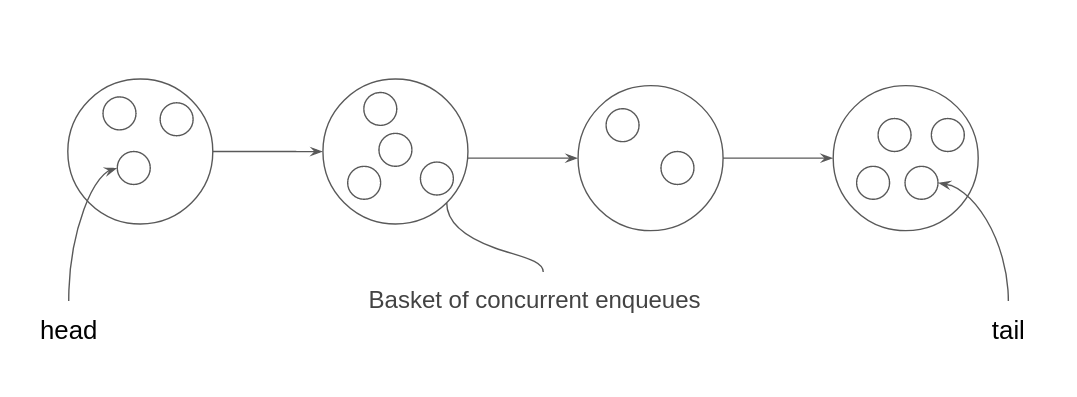
\includegraphics[scale=0.3]{pics/baskets}
  \caption{Baskets queue idea. There is a time that all operations in a basket were running concurrently, but only one has succeeded to do \texttt{CAS}. To order the operations in a basket, the mechanism in the algorithm for processes is to \texttt{CAS} again. The successful process will be the next one in the basket and so on.}
\end{figure}

Ladan-Mozes and Shavit~\cite{DBLP:journals/dc/Ladan-MozesS08} presented an Optimistic Approach to Lock-Free FIFO Queues. They use a doubly-linked list and do fewer \texttt{CAS} operations than MS-queue. But as before, the worst case is when there are $p$ concurrent enqueues which have to be enqueued one by one. The amortized worst-case complexity is still $\Omega(p)$ \texttt{CAS}es.

Hendler et al.~\cite{DBLP:conf/spaa/HendlerIST10} proposed a new paradigm called flat combining. Their queue is linearizable but not lock-free. Their main idea is that with knowledge of all the history of operations, it might be possible to answer queries faster than doing them one by one. In our work we also maintain the whole history. They present experiments that show their algorithm performs well in some situations.

Gidenstam, Sundell, and Tsigas~\cite{DBLP:conf/opodis/GidenstamST10} introduced a new algorithm using a linked list of arrays. Global head and tail pointers point to arrays containing the first and last elements in the queue. Global pointers are up to date, but head and tail pointers may be behind in time. An enqueue or a dequeue searches in the head array or tail array to find the first unmarked element or last written element (see~Figure~\ref{fig::sundell}). Their data structure is lock-free. Still, if the head array is empty and $p$ processes try to enqueue simultaneously, the step complexity remains $\Omega(p)$.

\begin{figure}[hbt]
  \center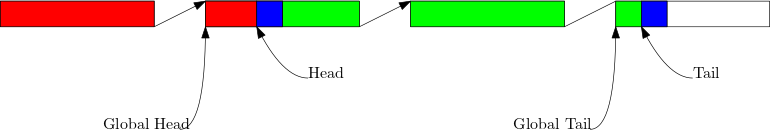
\includegraphics[scale=0.5]{pics/sundell}
    \caption{\label{fig::sundell}Global pointers point to arrays. Head and Tail elements are blue, dequeued elements are red and current elements of the queue are green.}
\end{figure}

Kogan and Petrank~\cite{DBLP:conf/ppopp/KoganP11} introduced wait-free queues based on the MS-queue and use Herlihy's helping technique to achieve wait-freedom. Their step complexity is $\Omega(p)$ because of the helping mechanism.

%todo: comparison
%Milman et al.~\cite{DBLP:conf/spaa/MilmanKLLP18} designed BQ: A Lock-Free Queue with Batching. Their idea of batching allows a sequence of operations to be submitted as a batch for later execution. It supports a new notion introduced by the authors called Extended Medium Futures Linearizability.

%Nikolaev and Ravindran~\cite{DBLP:journals/corr/abs-2201-02179} wCQ to be completed.
In the worst-case step complexity of all the list-based queues discussed above, there is a $p$ term that comes from the case all $p$ processes try to do an enqueue simultaneously. Morrison and Afek call this the \textit{CAS retry problem}~\cite{DBLP:conf/ppopp/MorrisonA13}. It is not limited to list-based queues and array-based queues share the CAS retry problem as well~\cite{DBLP:conf/spaa/TsigasZ01,DBLP:conf/icdcn/Shafiei09,DBLP:conf/iceccs/ColvinG05} . We are focusing on seeing if we can implement a queue in sublinear steps in terms of $p$ or not.

\subsection{Universal Constructions}
Herlihy discussed the possibility of implementing shared objects from other objects~\cite{10.1145/114005.102808}. A \textit{universal construction} is an algorithm that can implement a shared version of any given sequential object. We can implement a concurrent queue using a universal construction. Jayanti proved an $\Omega(\log p)$ lower bound on the worst-case shared-access time complexity of $p$-process universal constructions~\cite{DBLP:conf/podc/Jayanti98a}. He also introduced a construction that achieves $\textsc{O}(\log^2 p)$ shared accesses~\cite{DBLP:conf/podc/ChandraJT98}. His universal construction can be used to create any data structure, but its implementation is not practical because of using unreasonably large-sized \texttt{CAS} operations.

Ellen and Woelfel introduced an implementation of a Fetch\&Inc object with step complexity of $O(\log p)$ using $O(\log n$)-bit \texttt{LL/SC} objects, where $n$ is the number of operations~\cite{10.1007/978-3-642-41527-2_20}. Their idea has similarities to Jayanti's construction, and they represent the value of the Fetch\&Inc using the history of successful operations. 

%FIFO queues have a wide range of use in OS and applications. The current state-of-the-art queues are implemented using linked lists; that's why they have factor p in their time complexity.

%\href{https://docs.google.com/spreadsheets/d/1cL1tgXXdljkh462sMwkTVMHH_k0MBTmslIVM3xA5VS4/edit#gid=0}{Table of previous works}

%There is a connection between queues and universal constructions. We can implement a universal construction using a queue. We can store operations in the shared queue and compute operations' responses using the queue's content. Some impractical universal constructions are using big words as "...".

\subsection{Attiya Fourier Lower Bound}
\pagebreak

\pagebreak
\section{Our Queue}
Jayanti and Petrovic introduced a wait-free polylogarithmic multi-enqueuer single-dequeuer queue~\cite{DBLP:conf/fsttcs/JayantiP05}. We benefit from some ideas of their work to design a a polylogarithmic multi-enqueuer multi-dequeuer queue. Our algorithm despite them does not use \texttt{CAS} operations with big words and does not put a limit on the number of concurrent operations. I our model there are $p$ procesess doing \nf{Enqueue(),Dequeue()} operations concurrently. We use a shared tree among the processes (see Figure~\ref{fig::blocktree}) to agree on one total ordering on the operations invoked by processes. Each process has a leaf which the order of operations invoked by the process is stored in it. When a process wishes to do an operation it appends the operation to its leaf and then tries to propagate its new operation up to the tree's root. In each node the ordering of operations propagated up to it is stored. All processes agree on the sequence stored in the root and it is defined to be the linearization ordering. 
\begin{figure}[hbt]
\begin{center}
\Tree [ [ [ $P_1$ $P_2$ ] [ $P_3$ $P_4$ ] ]
          [ [ $P_5$ $P_6$ ] [ $P_7$ $P_8$ ] ] ]
\end{center}
\caption{\label{fig::blocktree}Each process has a leaf and in each node there is an ordering of operations stored. Each node tries to propagate its operations up to the root, which stores the total ordering of all operations.}  
\end{figure}

\it{Add sequence to nodes}

We could implement the sequence stored in each node using an array of the queue operations and append some operations to the sequence by doing \tt{k-CAS} operation on the end of the array. To do a propagate step on node $n$ in the tree, we aggregate the operations from node $n$'s both children (that have not already been propagated to $n$) and try to append them into $n$. We call this procedure \sc{Refresh}$(n)$. The main idea is that if we call \sc{Refresh}$(n)$ twice, the operations in $n$'s children before the first \sc{Refresh}$(n)$ are guaranteed to be in $n$.
Because if both of the \sc{Refresh}$(n)$s fail to do \nf{k-CAS} then there is another instance of \nf{Refresh()} in between which has succeeded to do \nf{CAS} and has already appended the operations that the first \nf{Refresh} was trying to append. This mechanism makes us overcome the \nf{CAS} Retry Problem.

\begin{figure}[hbt]
\begin{center}
\begin{subfigure}[b]{.49\textwidth}
  \centering
  \resizebox{\columnwidth}{!}{
  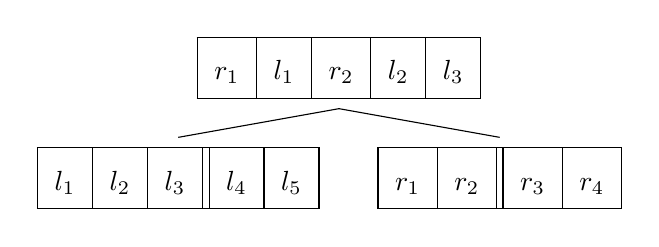
\begin{tikzpicture}[level 1/.style={level distance=1.4cm,sibling distance=0.5cm}]
\Tree [.{\begin{tabular}{|c|c|c|c|c|c|}  \hline $r_1$ & $l_1$ & $r_2$ & $l_2$ & $l_3$ \\ \hline \end{tabular}}
{\begin{tabular}{|c|c|c||c|c|}  \hline $l_1$ & $l_2$ & $l_3$ & $l_4$ & $l_5$ \\ \hline \end{tabular}}
{\begin{tabular}{|c|c||c|c|}  \hline $r_1$ & $r_2$ & $r_3$ & $r_4$\\ \hline \end{tabular}} ]
\end{tikzpicture}}
  \caption{Operations after $||$ are new.}
\end{subfigure}
\hfill
\begin{subfigure}[b]{.49\textwidth}
  \centering
  \resizebox{\columnwidth}{!}{
  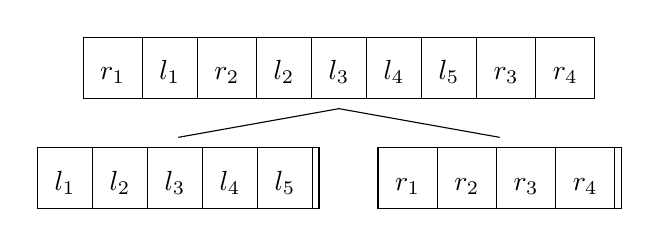
\begin{tikzpicture}[level 1/.style={level distance=1.4cm,sibling distance=0.5cm}]
\Tree [.{\begin{tabular}{|c|c|c|c|c|c|c|c|c|c|}  \hline $r_1$ & $l_1$ & $r_2$ & $l_2$ & $l_3$ & $l_4$ & $l_5$ & $r_3$ & $r_4$  \\ \hline \end{tabular}}
{\begin{tabular}{|c|c|c|c|c||}  \hline $l_1$ & $l_2$ & $l_3$ & $l_4$ & $l_5$ \\ \hline \end{tabular}}
{\begin{tabular}{|c|c|c|c||}  \hline$r_1$ & $r_2$ & $r_3$ & $r_4$\\ \hline \end{tabular}} ]
\end{tikzpicture}}
  \caption{New operations are added to the parent node.}
\end{subfigure}
\caption{\label{fig::propagstep} Before and after of a \sc{Refresh}$(n)$ with successful \nf{CAS}. Operations propagating from the left child are numbered with $l$ and from the right child by $r$ and the operations in children after $||$ are new.}
\end{center}
\end{figure}
\it{fix $||$}
\begin{figure}[h]
\begin{center}
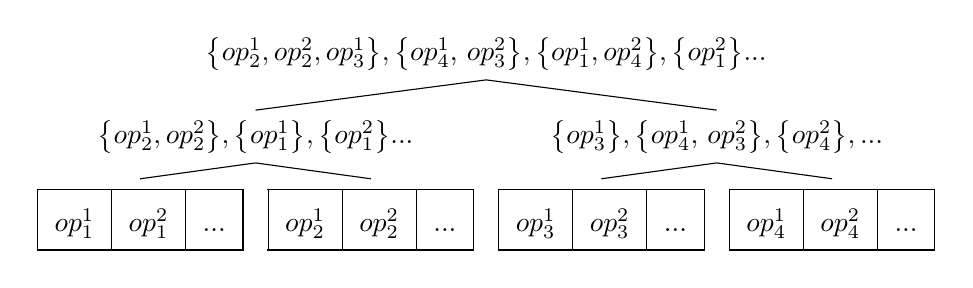
\begin{tikzpicture}
  
\Tree [.{$\big\{op_2^1,op_2^2,op_3^1\big\},\big\{op_4^1$, $op_3^2\big\},\big\{op_1^1, op_4^2\big\},\big\{op_1^2\big\}...$ }  [.{ $\big\{op_2^1, op_2^2\big\},\big\{op_1^1\big\},\big\{op_1^2\big\}...$ }
      {\begin{tabular}{|l|c|c|c}  \hline $op_1^1$ & $op_1^2$ & ... \\ \hline\end{tabular}} {\begin{tabular}{|l|c|c|c}  \hline $op_2^1$ & $op_2^2$ & ... \\ \hline\end{tabular}} ] [.{ $\big\{op_3^1\big\},\big\{op_4^1$, $op_3^2\big\},\big\{op_4^2\big\},...$ } {\begin{tabular}{|l|c|c|c}  \hline $op_3^1$ & $op_3^2$ & ... \\ \hline\end{tabular}} {\begin{tabular}{|l|c|c|c} \hline $op_4^1$ & $op_4^2$ & ... \\ \hline\end{tabular}} ] ]

\end{tikzpicture}
\caption{\label{fig::set} In each internal node, we store the set of all the operations propagated together, and one can arbitrarily linearize the sets of concurrent operations among themselves. Since we linearize operations when they are added to the root, ordering the blocks in the root is important.}
\end{center}
\end{figure}

The solution for  implementing the orderings in the tree told above is not efficient, because there are big \nf{CAS}es and operations information are copied all the way up to the root.
Instead of storing operations explicitly in the nodes, we can keep track of some statistics of them. This allows us to \texttt{CAS} fixed-size objects in each \textsc{Refresh}($n$). To do that, we introduce blocks that only contain the number of operations from the left and the right child in a \texttt{Refresh}() procedure and only propagate the statistics block of the new operations. In each \nf{Refresh()} there is at most one operation from each process trying to be propagated, because one operation cannot invoke two operations concurrently. Furthermore since the operations in a \textsc{Refresh()} step are concurrent we can linearize them  among themselves in any order we wish. Note that if two operations are in read one \textsc{Refresh()} step in a node they are going to be propagated up to the root together. Our choice is to put the operations propagated from the left child before the operations propagated from the right child. In this way if we know the number of operations from the left child and the number of operations from the right child in a block  we have a complete ordering on the operations.

A process may wish to know the $i$th propagated operation or the rank of a propagated operation in the linearization. In our case of implementing a queue, we can make an assumption that one process only wishes to know the rank of a dequeue and one tries to get an enqueue with its rank. \nf{enqueue}s and \nf{dequeue}s are appended to the tree and when we want to find the response to a \nf{dequeue}, we compute the place of the dequeue in the linearization and using the rank of the dequeue among deqeueues and some information stored in the root we compute which enqueue is the answer to the dequeue or if the answer is null. If the answer was some enqueue we find the enqueue using \texttt{DSearch(i)} and \nf{GetEnqueue(n,b,i)}. \texttt{DSearch(i)} finds the block containing the $i$th enqueue in the root and \nf{GetEnqueue(n,b,i)} finds its sub-block recursively to reach a leaf. \texttt{Index()} is similar but more complicated, finding super-blocks from a leaf to the root. The main challenge in each level of \texttt{Get(i)} and \texttt{Index(op)} is that it should take polylogarithmic steps with respect to $p$. After appending operation \texttt{op} to the root, processes can find out information about the linearization ordering using \texttt{Get(i)} and \texttt{Index(op)}. Each block stores an extra constant amount of information (like prefix sums) to allow binary searches to find the required block in a node quickly.

\paragraph{Implementing Queue using Block Tree}
In this work, we design a queue with $O(\log^2 p +\log n)$ steps per operation, where $n$ is the number of total operations invoked. We avoid the $\Omega(p)$ worst-case step complexity of existing shared queues based on linked lists or arrays (CAS Retry Problem). A queue stores a sequence of elements and supports two operations, enqueue and dequeue. \texttt{Enqueue(e)} appends element \texttt{e} to the sequence stored.\texttt{Dequeue()} removes and returns the first element among in the sequence. If the queue is empty it returns \texttt{null}. Knowing index $i$ is the tail of the queue, we can return the dequeue response using \texttt{Get(i)}.  So in the rest we modify block tree to compute \texttt{i} for each \texttt{Dequeue()} to achieve a FIFO queue.

\begin{figure}

\begin{center}
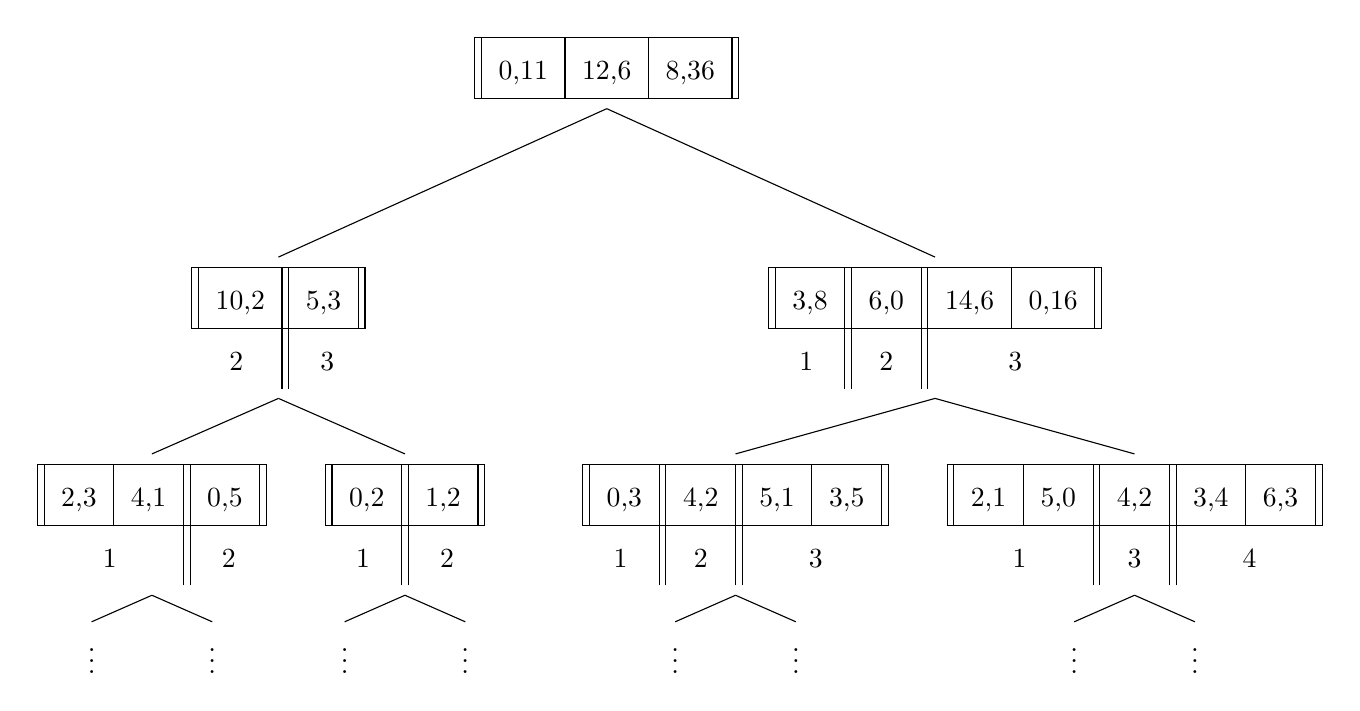
\begin{tikzpicture}[level 1/.style={level distance=3.3cm,sibling distance=1cm},
	level 2/.style={level distance=2.5cm,sibling distance=0.5cm},
	level 3/.style={level distance=1.8cm,sibling distance=1.2cm}]
  

\Tree [.{\begin{tabular}{||c|c|c||}  \hline 0,11 & 12,6 & 8,36 \\ \hline\end{tabular}}
 [.{\begin{tabular}{||c||c||}  \hline 10,2 & 5,3 \\  \hline \multicolumn{1}{c||}{2} & \multicolumn{1}{c}{3} \end{tabular}}
 [.{\begin{tabular}{||c|c||c||}\hline 2,3 & 4,1 & 0,5 \\\hline\multicolumn{2}{c||}{1} & \multicolumn{1}{c}{2}\end{tabular}} $\vdots$ $\vdots$ ]
  [.{\begin{tabular}{||c||c||}  \hline 0,2 & 1,2 \\  \hline \multicolumn{1}{c||}{1} & \multicolumn{1}{c}{2} \end{tabular}} $\vdots$ $\vdots$ ] ]
          [.{\begin{tabular}{||c||c||c|c||}  \hline 3,8 & 6,0 & 14,6 & 0,16 \\ \hline \multicolumn{1}{c||}{1} & \multicolumn{1}{c||}{2} & \multicolumn{2}{c}{3}\end{tabular}}
           [.{\begin{tabular}{||c||c||c|c||}  \hline 0,3 & 4,2 & 5,1 & 3,5 \\ \hline \multicolumn{1}{c||}{1} & \multicolumn{1}{c||}{2}& \multicolumn{2}{c}{3}\end{tabular}} $\vdots$ $\vdots$ ]
            [.{\begin{tabular}{||c|c||c||c|c||}  \hline 2,1 & 5,0 & 4,2 & 3,4 & 6,3 \\ \hline \multicolumn{2}{c||}{1} & \multicolumn{1}{c||}{3} & \multicolumn{2}{c}{4}\end{tabular}} $\vdots$ $\vdots$ ] ] ]

\end{tikzpicture}
\end{center}
\caption{\label{fig:block} Showing concurrent operation sets with blocks. Each block consists of a pair(left, right) indicating the number of operations from the left and the right child, respectively. Block (12,6) in the root contains blocks (10,2) from the left child and (6,0) from the right child. Blocks between two lines $||$ are propagated together to the parent. For example, Blocks (2,3) and (4,1) from the leftmost leaf and (0,2) from its sibling are propagated together into the block (10,2) in their parent. The number underneath a group of blocks in a node indicates which block in the node's parent those blocks were propagated to. Each block $b$ in node $n$ is the aggregation of blocks in the  children of $n$ that are newly read by the\textsc{Propagate}() step that created block $b$. For example, the third block in the root (8,36) is created by merging block (5,3) from the left child and (14,6) and (0,16) from the right child. Block (5,3) also points to elements from blocks (0,5) and (1,2). We choose to linearize operations in a block from the left child before those from the right child as a convention. Operations within a block of the root can be ordered in any way that is convenient. In effect, this means that if there are concurrent new blocks in a \textsc{Refresh}() step from several processes we linearize them in the order of their process ids. So for example  operations aggregated in block (10,2) are in the order (2,3),(4,1),(0,2). All blocks from the left child with come before the right child and the order of blocks of each child is preserved among themselves.
}
\end{figure}

\paragraph{}
\textsc{GetIndex}($i$) returns the $i$th operation stored in the block tree sequence. We do that by finding the block $b_i$ containing $i$th element in the root, and then recursively finding the subblock of $b_i$ which contains $i$th element. To make this recursive search faster, instead of iterating over all elements in sequence of blocks we store prefix sum of number of elements in the blocks sequence and pointers to make BinarySearch faster.

Furthermore, in each block, we store the prefix sum of left and right elements. Moreover, for each block, we store two pointers to the last left and right subblock of it (see fig \ref{fig::pointer} and \ref{fig:prefix}).

\begin{figure}
\begin{center}
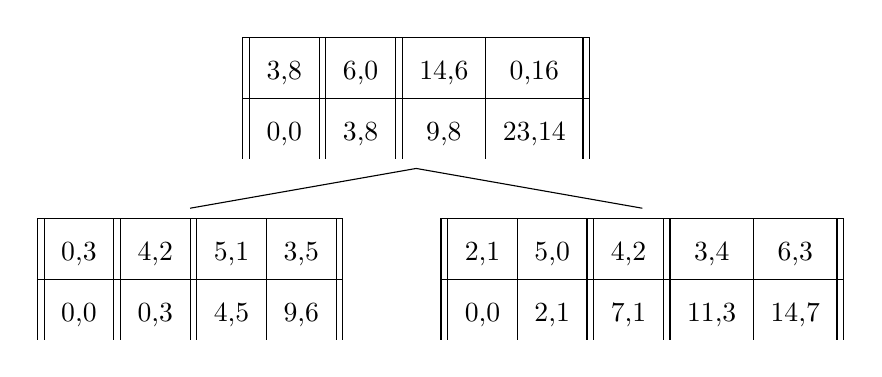
\begin{tikzpicture}[level 1/.style={level distance=2.3cm,sibling distance=1cm}]
  
\Tree [.{\begin{tabular}{||c||c||c|c||}  \hline 3,8 & 6,0 & 14,6 & 0,16 \\ \hline  0,0 & 3,8 & 9,8 & 23,14\end{tabular}}
           [.{\begin{tabular}{||c||c||c|c||}  \hline 0,3 & 4,2 & 5,1 & 3,5 \\ \hline 0,0 & 0,3 & 4,5 & 9,6 \end{tabular}} ]
            [.{\begin{tabular}{||c|c||c||c|c||}  \hline 2,1 & 5,0 & 4,2 & 3,4 & 6,3 \\ \hline 0,0 & 2,1 & 7,1 & 11,3 & 14,7 \end{tabular}} ] ]


\end{tikzpicture}
\end{center}
\caption{\label{fig:prefix} Using Prefix sums in blocks. When we want to find block b elements in its children, we can use binary search. The number below each block shows the count of elements in the previous blocks.}
\end{figure}

\begin{figure}[hbt]
\centering
  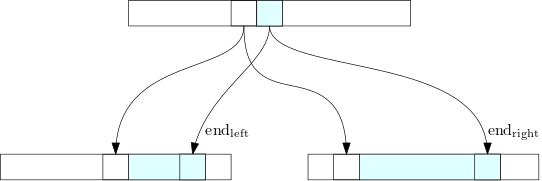
\includegraphics[width=5in]{pics/pointers}
  \caption{Block have pointers to the starting block of theirs for each child. \label{fig::pointer}}
\end{figure}


\paragraph{}
Starting from the root, \textsc{GetIndex}($i$) BinarySearches $i$ in the prefix sum array to find block containing $i$th operation, then continues recursively calling \textsc{GetElement}($b,i$) to find $i$th element of block $b$. From lemma $\ref{lem:block_size}$ we know a block size is at most $p$. So BinarySearch takes at most \textsc(O)$(\log p)$, since  with knowing pointers of a block and its previous block we can determine the base \texttt{(domain ?)} to search and its size is \textsc{O}$(p)$.



\paragraph{\texttt{CreateBlock()}} \texttt{CreateBlock(n)} returns a block containing new operations of \texttt{n}'s children. \texttt{b\textsuperscript{$\prime$}.end\textsubscript{left}} stores the index of the rightmost subblock of left child of \texttt{b}'s previous block. Other attributes are assigned values followed by definition.
\begin{figure}[hbt]
  \center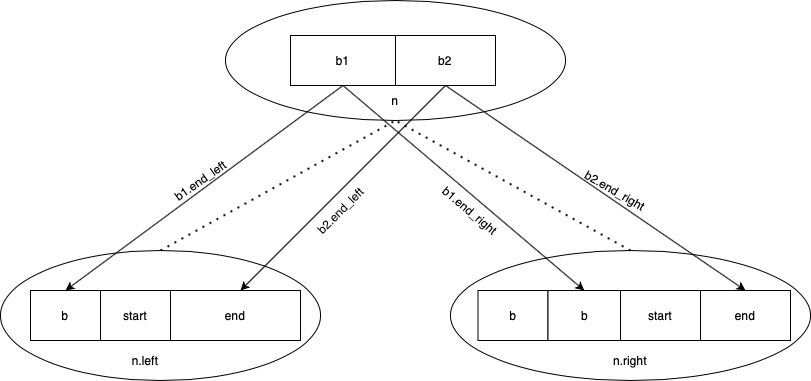
\includegraphics[width=5.5in]{pics/createblock}
  \caption{\label{fig::createBlock}Snapshot of a CreateBlock()}
\end{figure}

\begin{figure}[hbt]
  \center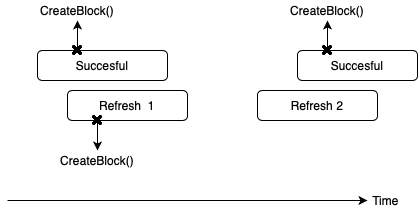
\includegraphics[width=4in]{pics/doublerefresh.png}
  \caption{The second failed Refresh is assuredly concurrent to a Successful \texttt{Refresh()} with \texttt{CreateBlock} line after first failed \texttt{Refresh}'s \texttt{CreateBlock()}.}
\end{figure}

\paragraph{Computing \texttt{Get(n, b, i)}}

\paragraph{How \texttt{Refresh(n)} works.}

\paragraph{Computing superblock}

 Let $i$ be the value $R_n$, a successful instance of \nf{Refresh()} on node \nf{n} reads from \nf{$n$.head}. $R_n$ does a successful \nf{CAS(null, $b$)} into \nf{n.blocks[$i$]}. Let $p$ be $n$\nf{}.parent. Without loss of generality for the rest of this section assume ${n}$ is the left child of $p$. From Lemma \ref{lem::appendExactlyOnce} we know there could be only one \nf{p.Refresh()} propagating $b$. Let $R_p$ be the first successful \nf{p.Refresh()} that reads some value greater than ${i}$ for \nf{left.head} and contains ${b}$ in its created block in Line \ref{invokeCreateBlock}. Let the index of the block $R_p$ put in $p$\nf{.blocks} be $j$.
 
Since the index of the superblock of ${b}$ is not known until $b$ is propagated, $R_n$ cannot set the \nf{super} field of ${b}$ while creating it. One approach is to set the \nf{super} field of ${b}$ by $R_n$ after propagating $b$ to $p$. This solution would not be efficient because there might be $p$ subblocks in the block $R_p$ propagated needing to update the \nf{super} field. However intuitively, once $b$ is installed, its superblock is going to be close to \nf{$n$.parent.head} at the time of installation. One idea is that if we know the approximate position of the superblock of $b$ then we can search for the real superblock when we wished to know the superblock of $b$ i.e. \nf{b.super} does not have to be the exact location of  the superblock of $b$, but we want it to be close to \nf{j}. We can set \nf{$b$.super} to \nf{$n$.parent.head} while creating $b$, but the problem is that there might be many \nf{$p$.Refresh}es that could happen after reading $p$\nf{.head} by $R_n$ and before propagating $b$ to $p$. If we set \nf{$b$.super} to \nf{$p$.head} after appending $b$ to \nf{$n$.blocks} (Line \ref{setSuper1}), $R_n$ might go to sleep at some time after installing $b$ and before setting \nf{$b$.super}. In this case the next \nf{Refresh}es on $n$ and \nf{n.parent} help fill in the value of \nf{$b$.super}.

Block $b$ is appended to \nf{n.blocks[h]} on Line \ref{cas}. After appending $b$, \nf{b.super} is set on Line \ref{setSuper1} of a call to \nf{Advance} from \nf{$n$.Refresh()} by the same process or another process or  maybe an \nf{$n$.parent.Refresh()}. We want to bound how far \nf{b.super} is from the index of $b$'s superblock, which is created by a successful \nf{n.parent.Refresh()} that propagates $b$.


%\subsection{What should a \texttt{Dequeue()} return, regarding history of operations?}
\paragraph{Queue from tree}
Now, we describe how to use the tree to implement a queue. Consider the following execution of operations. \texttt{Enqueue(e)} appends an operation with input argument \texttt{e} in the block tree. What should a \texttt{Dequeue()} return? To compute the response of a \texttt{Dequeue()}, process $p$ first appends a \texttt{DEQ} operation to the tree. Then $p$ finds the rank of the \texttt{DEQ} using \texttt{Index()}, the rank of the \texttt{DEQ} and the information stored in the root about the queue $p$ computes the rank of  the \texttt{ENQ} having the answer of the \texttt{DEQ}. Finally $p$ returns the argument of that \texttt{ENQ} using \texttt{Get(i)}.

\begin{table}[hbt]
\centering
  \begin{tabular}{c|c|c|c|c|c|c|c|c|c}
    \hline \texttt{ENQ(5)}& \texttt{ENQ(2)}& \texttt{DEQ()}& \texttt{ENQ(3)}&\texttt{DEQ()}& \texttt{DEQ()}& \texttt{DEQ()}& \texttt{ENQ(4)}& \texttt{ENQ(6)}& \texttt{DEQ()}\\ \hline
  \end{tabular}
  \caption{An example histoy of operations on the queue}
\end{table}



\paragraph{}
A non-null dequeue is one that returns a non-null value. In the example above, \texttt{Dequeue()} operations return \texttt{5, 2, 3, null, 4} in order. Before \texttt{ENQ(4)} the queue gets empty so the last \texttt{DEQ()} returns null. If the queue is non-empty and $r$ \texttt{Dequeue()} operations have returned a non-null response, then $i$th \texttt{Dequeue()} returns the input of the $r+1$th \texttt{Enqueue()}. So, in order to answer a Dequeue, it's sufficent to know the size of the queue and the number of previous non-null dequeues.

%\texttt{DEQ[i] = (size>0) ? ENQ[r+1] : null;}


%\subsection{What should a \texttt{Dequeue()} return, regarding history of blocks of operations?}

\paragraph{}
In the Block Tree, we did not store the sequence of operations explicitly but instead stored blocks of concurrent operations to optimize \texttt{Propagate()} steps and increase parallelism. So now the problem is to find the result of each Dequeue. From lemma \ref{lem:block_size} we know we can linearize operations in a block in any order; here, we choose to decide to put Enqueue operations in a block before Dequeue operations. In the next example, operations in a cell are concurrent. \texttt{DEQ()} operations return \texttt{null, 5, 2, 1, 3, 4, null} respectively. We will next describe how these values can be computed efficiently.

\begin{table}[hbt]
\centering
  \begin{tabular}{c|c|c|c}
    \hline \texttt{DEQ()} & \texttt{ENQ(5)}, \texttt{ENQ(2)}, \texttt{ENQ(1)}, \texttt{DEQ()}& \texttt{ENQ(3)}, \texttt{DEQ()}&  \texttt{ENQ(4)}, \texttt{DEQ()}, \texttt{DEQ()}, \texttt{DEQ()}, \texttt{DEQ()}\\ \hline
  \end{tabular}
  \caption{An example history of operation blocks on the queue}
\end{table}


\paragraph{}
Now, we claimed that by knowing the current size of the queue and the number of non-null dequeue operations before the current dequeue, we could compute the index of the resulting \texttt{Enqueue()}. We apply this approach to blocks; if we store the size of the queue after each block of operations happens and the number of non-null dequeues dequeues till a block, we can compute each dequeue's index of result in \textsc{O}$(1)$ steps.

\begin{table}[hbt]
\centering
  \begin{tabular}{c|c|c|c|c}
    \hline &\texttt{DEQ()} & \texttt{ENQ(5)}, \texttt{ENQ(2)}, \texttt{ENQ(1)}, \texttt{DEQ()}& \texttt{ENQ(3)}, \texttt{DEQ()}&  \texttt{ENQ(4)}, \texttt{DEQ()}, \texttt{DEQ()}, \texttt{DEQ()}, \texttt{DEQ()}\\ \hline
    \#enqueues & 0 & 3 & 1 & 1 \\ \hline
        \#dequeues & 1 & 1 & 1 & 4 \\ \hline
            \#non-null dequeues & 0 & 1 & 2 & 5 \\ \hline
                size & 0 & 2 & 2 & 0 \\ \hline
  \end{tabular}
  \caption{Augmented history of operation blocks on the queue}
\end{table}

%\begin{definition}
%  \texttt{index(op)}: index of the given Dequene among same type operation in conataing block.
%  
%  \texttt{INDEX(op)}: index of the given Dequene among same type operation in all operations.
%  
%\end{definition}

Size and the number of non-null dequeues for $b$th block could be computed this way:\\
\texttt{size[b]= max(size[b-1] +enqueues[b] -dequeues[b], 0)}\\
\texttt{non-null dequeues[b]= non-null dequeues[b-1] +dequeues[b] -size[b-1] -enqueues[b]}

Given \texttt{DEQ} is in block \texttt{b}, \texttt{response(DEQ)} would be:\\
\texttt{(size[b-1]- index of DEQ in the block's dequeus >=0) ? ENQ[non-null dequeus[b-1]+ index of DEQ in the block's dequeus] : null;}


\begin{figure}[hbt]
\centering
  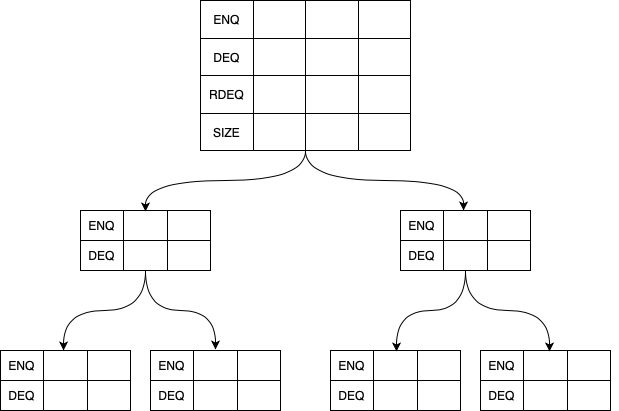
\includegraphics[width=5in]{pics/queue}
  \caption{Fields stored in the Queue nodes. \label{fig::queue}}
\end{figure}


\subsection{Pseudocode description}

\paragraph{Specification}
A Queue is a shared data structure that stores a sequence of elements. It has two methods \texttt{Enqueue(e)} and \texttt{Dequeue()}. \texttt{Enqueue(e)} adds \texttt{e} to the end of the sequence. \texttt{Dequeue()} returns the first element stored in the sequence and removes it from the sequence.

\paragraph{Tree}
In order to reach an agreement on the order of operations among $p$ processes, we use a Tournament Tree. Leaf \texttt{l\textsubscript{i}} is assigned to a process \texttt{i}. Each process adds $op$ to its leaf. In each internal node an ordering of operations in its subtree is stored. All processes agree on the total ordering of all operations stored in the root. This ordering will be the linearization of the operations.
\paragraph{Implicit Storing Blocks}
For efficiency, instead of storing explicit sequence of operations in nodes of the Tournament Tree, we use Blocks. A Block is a constant size object that implicitly represents a sequence of operations. In each node there is an array of Blocks.

Block $b$ contains subblocks in the left and right children. WLOG left subblocks of $b$ are some consecutive blocks in the left child starting from where previous block of $b$ has ended to the the end of $b$. See Figure \ref{fig::createBlock} .

We store ordering among \texttt{operation}s in the tournament tree constructed by \texttt{node}s. In each \texttt{node} we store pointers to its relatives, an array of \texttt{block}s and an index to the first empty \texttt{block}. Furthermore in \texttt{leaf} nodes there is an array of \texttt{operations} where each \texttt{operation} is stored in one cell with the same index in \texttt{blocks}. There is a \texttt{counter} in each \texttt{node} incrementing after a successful \texttt{Refresh()} step. It means after that some bunch of \texttt{block}s in a node have propagated into the parent then the \texttt{counter} increases. Each new \texttt{block} added to a node sets its \texttt{time} regarding \texttt{counter}. This helps us to know which blocks have aggregated together to a block, not precisely though. We also store the index of the aggregated \texttt{block} of a \texttt{block} with \texttt{time} $i$ in \texttt{super[i]}. 

In each \texttt{block} we store 4 essential stats that implicitly summarize which operations are in the block \texttt{num\textsubscript{enq-left}}, \texttt{num\textsubscript{deq-left}}, \texttt{num\textsubscript{enq-right}}, \texttt{num\textsubscript{deq-right}}. In order to make \texttt{BinarySearch()}es faster we store prefix sums as well and there are some more general stats that help to make pseudocode more readable but not necessary.

To compute the head of the \texttt{queue} before a \texttt{dequeue} two more fields are stored in the root \texttt{size} and \texttt{sum\textsubscript{non-null deq}}. \texttt{size} in a \texttt{block} shows the number of elements after the \texttt{block} has finished and \texttt{sum\textsubscript{non-null deq}} is the total number of non-null dequeues till the \texttt{block}.

\texttt{Enqueue(e)} just \texttt{append}s an \texttt{operation} with \texttt{element e} to the \texttt{root}. \texttt{Dequeue()} appends an \texttt{operation} to the root and computes its ordering and the \texttt{enqueue operation} containing the head before it calling \texttt{ComputeHead()} and then \texttt{gets} and returns the \texttt{operation}'s element.

\texttt{Append(op)} adds \texttt{op} to the invoking process's leaf's \texttt{ops} and \texttt{blocks}, \texttt{propagate}s it up to the root and if the \texttt{op} is a dequeue returns its order in residing block in the root and the block's index. As we said later \texttt{Propagate()} assuredly aggregates new blocks to a block in the parent by calling \texttt{Refresh()} two times. \texttt{Refresh(n)} creates a block, tries to CAS it into the p\texttt{n}'s \texttt{blocks} and if it was successful updates \texttt{super} and \texttt{counter} in both of \texttt{n}'s children.

We only want to know the \texttt{element} of \texttt{enqueue} operations and compute ordering for \texttt{dequeue} operations. That's the reason here \texttt{Get()} searches between enqueues only and \texttt{Index()} returns ordering of a dequeue among dequeues. \texttt{Get(n, b ,i)} decides the requested element is in which child of n and continues to search recursively. \texttt{index(n, i, b)} calculates the ordering of the given operation in \texttt{n}'s parent each step and finally returns the result among total ordering.

\pagebreak
\newpage
\newgeometry{left=0.6in,right=0.6in,top=0.6in,bottom=0.8in}

\subsection{Pseudocode}
\begin{algorithm}
\caption{Tree Fields Description}
\begin{algorithmic}[1]
\setcounter{ALG@line}{100}
\begin{multicols}{2}

\Statex $\diamondsuit$ \tt{\sl{Shared}}
\begin{itemize}
\item \textsf{A binary tree of \tt{Node}s with one \tt{leaf} for each process. \tt{root} is the root \nf{node}.}
\end{itemize}

\Statex $\diamondsuit$ \tt{\sl{Local}}
\begin{itemize}
\item \tt{\sl{Node} leaf:} \sf{ process's leaf in the tree.}
\end{itemize}

\Statex $\blacktriangleright$ \tt{\sl{Node}}
\begin{itemize}
\item \tt{\sl{*Node} left, right, parent} \textsf{: Initialized  when creating the tree.}
\item \tt{\sl{Block[]} blocks} \textsf{: Initially \tt{blocks[0]} contains an empty block with all fields equal to 0.}
\item \tt{\sl{int} \head= 1}\textsf{: \#\tt{block}s in \tt{blocks}. \tt{blocks[0]} is a block with all integer fields equal to zero.}
\end{itemize}

\Statex $\blacktriangleright$ \tt{\sl{Block}} 

\begin{itemize}
  \item \tt{\sl{int} super}
  \textsf{: approximate index of the superblock, read from \tt{parent.head} when appending the block to the node}
\end{itemize}

\Statex $\blacktriangleright$ \tt{\sl{LeafBlock} extends \sl{Block}}
\begin{itemize}
  \item \tt{\sl{Object} element}
  \textsf{: Each block in a leaf represents a single operation. If the operation is \tt{enqueue(x)} then \tt{element=x}, otherwise \tt{element=null}.}
  
    \item \tt{\sl{int} sum\sub{enq}, sum\sub{deq}}
  \textsf{: \# enqueue, dequeue operations in the prefix for the block}
  
\end{itemize}

\pagebreak

\Statex $\blacktriangleright$ \tt{\sl{InternalBlock} extends \sl{Block}}
\begin{itemize}
    \item \tt{\sl{int} end\sub{left}, end\sub{right}}
  \textsf{:~~indices of the last subblock of the block in the left and right child}
  \item \tt{\sl{int} sum\sub{enq-left}}
  \textsf{: \# enqueue operations in the prefix for \tt{left.blocks[end\sub{left}]}}
  \item \tt{\sl{int} sum\sub{deq-left}}
  \textsf{: \# dequeue operations in the prefix for \tt{left.blocks[end\sub{left}]}}
  \item \tt{\sl{int} sum\sub{enq-right}}
  \textsf{: \# enqueue operations in the prefix for \tt{right.blocks[end\sub{right}]}}
  \item \tt{\sl{int} sum\sub{deq-right}}
  \textsf{: \# dequeue operations in the prefix for \tt{right.blocks[end\sub{right}]}}
\end{itemize}


\Statex $\blacktriangleright$ \tt{\sl{RootBlock} extends \sl{InternalBlock}}
\begin{itemize}
  \item \tt{\sl{int} \size}
  \textsf{: size of the queue after performing all operations in the prefix for this block}
\end{itemize}

\end{multicols}
\end{algorithmic}
\end{algorithm}

\begin{footnotesize}

\it{Abbreviations:}
\begin{itemize}
 \item \tt{blocks[b].sum\sub{x}=blocks[b].sum\sub{x-left}+blocks[b].sum\sub{x-right}}  \tt{ (for b$\geq$0 and x $\in$ \{enq, deq\}})
 \item \tt{blocks[b].sum=blocks[b].sum\sub{enq}+blocks[b].sum\sub{deq}}  \tt{ (for b$\geq$0})
  \item \tt{blocks[b].num\sub{x}=blocks[b].sum\sub{x}-blocks[b-1].sum\sub{x}} \\ \tt{(for b>0 and x $\in$ \{$\emptyset$, enq, deq, enq-left, enq-right, deq-left, deq-right\})}
\end{itemize}
\end{footnotesize}

\pagebreak

\begin{algorithm}
\caption{\tt{\sl{Queue}}}
\begin{algorithmic}[1]
\setcounter{ALG@line}{200}


\Function{void}{Enqueue}{\sl{Object} e} \cmt{Creates a \tt{block} with element \tt{e} and adds it to the tree.}
\State \tt{block newBlock= \Call{new}{\sl{LeafBlock}}}
\State \tt{newBlock.element= e}
\State \tt{newBlock.sum\sub{enq}= leaf.blocks[leaf.\head].sum\sub{enq}+1}
\State \tt{newBlock.sum\sub{deq}= leaf.blocks[leaf.\head].sum\sub{deq}}
\State \tt{leaf.}\Call{Append}{newBlock}
\EndFunction{Enqueue}

\Statex

\Function{Object}{Dequeue()}{} \cmt{Creates a block with null value element, appends it to the tree, computes its order among operations, and returns its response.}
\State \tt{block newBlock= \Call{new}{\sl{LeafBlock}}} 
\State \tt{newBlock.element= null}
\State \tt{newBlock.sum\sub{enq}= leaf.blocks[leaf.\head].sum\sub{enq}}
\State \tt{newBlock.sum\sub{deq}= leaf.blocks[leaf.\head].sum\sub{deq}+1}
\State \tt{leaf.}\Call{Append}{newBlock}
\State \tt{<b, i>=} \Call{IndexDequeue}{leaf.\head, 1}
\State \tt{output=} \Call{FindResponse}{b, i} 
\label{deqRest}
\State \Return{\tt{output}}
\EndFunction{Dequeue}

\Statex

\Function{<int, int>}{FindResponse}{\sl{int} b, \sl{int} i}\cmt{Returns the the response to the $D_{root,b,i}$.}
\If{\tt{ root.blocks[b-1].\size}\tt{ + root.blocks[b].num\sub{enq} - i $<$ 0}} \label{checkEmpty}\cmt{Check if the queue is empty.}
\State \Return \tt{null} \label{returnNull}
\Else
\State \tt{e= i - root.blocks[b-1].size + root.blocks[b-1].sum\sub{enq}} \label{computeE}
\cmt{$E_e(root)$ is the response.}
\State \Return \tt{root.GetEnqueue(root.\Call{DSearch}{e, b})}\label{findAnswer}
\EndIf
\EndFunction{FindResponse}

\end{algorithmic}
\end{algorithm}

\begin{algorithm}
\caption{Root}
\begin{algorithmic}[1]
\setcounter{ALG@line}{800}
\Statex
\Statex $\leadsto$ \textsf{Precondition: \tt{root.blocks[end].sum\sub{enq} $\geq$ \tt{e}}}
\Function{<int, int>}{DSearch}{\sl{int} e, \sl{int} end}
\cmt{Returns \tt{<b,i>} if $E_e(root)=E_i(root,b)$.}
\State \tt{start= end-1} \label{dsearchStart}
\While{\tt{root.blocks[start].sum\sub{enq}}$\geq$\tt{e}}
\State \tt{start= max(start-(end-start), 0)} \label{doubling}
\EndWhile \label{dsearchEnd}
\State \tt{b= root.BinarySearch(sum\sub{enq}, e, start, end)} \label{dsearchBinarySearch}
\State \tt{i= e- root.blocks[b-1].sum\sub{enq}} \label{DSearchComputei}
\State\Return \tt{<b,i>}
\EndFunction{DSearch}
\end{algorithmic}
\end{algorithm}

\begin{algorithm}
\caption{Leaf}
\begin{algorithmic}[1]
\setcounter{ALG@line}{600}

\Function{void}{Append}{\sl{block} blk} \cmt{Append is only called by the owner of the leaf.}
\State \tt{blocks[\head]= blk} 
\State \tt{\head+=1} \label{appendEnd} 
\State \tt{parent.}\Call{Propagate()}{} 
\EndFunction{Append}

\end{algorithmic}
\end{algorithm}

\pagebreak

\begin{algorithm}
\caption{\tt{\sl{Node}}}
\begin{algorithmic}[1]
\setcounter{ALG@line}{300}
\begin{multicols}{2}

\Function{void}{Propagate()}{}
\If{\bf{not} \Call{Refresh()}{}} \label{firstRefresh}
\State \Call{Refresh()}{} \label{secondRefresh}
\EndIf
\If{\tt{this} \bf{is not} \tt{root}}
\State \tt{parent.}\Call{Propagate()}{}
\EndIf
\EndFunction{Propagate}

\Statex

\Function{boolean}{Refresh()}{}
\State \tt{h= \head} \label{readHead}
\ForEach{\tt{dir} {\keywordfont{in}} \tt{\{left, right\}}} \label{startHelpChild1}
\State \tt{h\sub{dir}= dir.\head} \label{readChildHead}
\If{\nf{dir.blocks[h\sub{dir}]!=null}} \label{ifHeadnotNull}
\State{\tt{dir.\Call{Advance}{h\sub{dir}, h}}} \label{helpAdvance}
\EndIf
\EndFor \label{endHelpChild1}
\State \tt{new= \Call{CreateBlock}{h}} \label{invokeCreateBlock}
\If{\tt{new.num==0}} \Return{\tt{true}} \label{addOP} 
\EndIf
\State{\tt{result= blocks[h].CAS(null, new)}} \label{cas}

\State \tt{h\sub{p}= parent.\head} \label{readParentHead}
\State{\tt{this.\Call{Advance}{h, h\sub{p}}}} \label{advance}
\State \Return{ \tt{result}}

\EndFunction{Refresh}

\Statex

\Function{void}{Advance}{\sl{int} h, \sl{int} hp}

\State \tt{blocks[h].super.CAS(null, hp)} \label{setSuper1}
\State \tt{head.CAS(h, h+1)} \label{incrementHead}
\EndFunction{Advance}

\pagebreak
\Statex $\leadsto$ \textsf{Precondition: \tt{blocks[start..end]} contains a block with field \tt{f} $\geq$ \tt{i}}
\Function{int}{BinarySearch}{\sl{field} f, \sl{int} i, \sl{int} start, \sl{int} end}

\Statex \cmt{\textmd{Does binary search for~the value \tt{i} of the given prefix sum \tt{field}. Returns the index of the leftmost block in \tt{blocks[start..end]} whose \sl{field} \tt{f} is $\geq$ \tt{i}}.}
%\State \Return \tt{result block's index}
\EndFunction{BinarySearch}

\Statex

\Function{<Block, int, int>}{CreateBlock}{\sl{int} i} 
\cmt{Creates and returns the block to be inserted as $i$th \tt{block} in \tt{blocks}.}
\State \tt{block newBlock= \Call{new}{\sl{block}}}
\ForEach{\tt{dir} {\keywordfont{in}} \tt{\{left, right\}}}
\State \tt{index\sub{last}= dir.\head-1} \label{lastLine}
\State \tt{index\sub{prev}= blocks[i-1].end\sub{dir}} \label{prevLine}
\State \tt{newBlock.end\sub{dir}= index\sub{last}} \label{endDefLine}
\State \tt{block\sub{last}= dir.blocks[index\sub{last}]}
\State \tt{block\sub{prev}= dir.blocks[index\sub{prev}]}
\State \cmt{\tt{newBlock} includes \tt{dir.blocks[index\sub{prev}+1..index\sub{last}]}.}
\State \tt{newBlock.sum\sub{enq-dir}= blocks[i-1].sum\sub{enq-dir} + block\sub{last}.sum\sub{enq} - block\sub{prev}.sum\sub{enq}} \label{setSumEnqLeft}
\State \tt{newBlock.sum\sub{deq-dir}= blocks[i-1].sum\sub{deq-dir} + block\sub{last}.sum\sub{deq} - block\sub{prev}.sum\sub{deq}} \label{setSumEnqRight}
\EndFor
\If{\tt{this} \bf{is} \tt{root}}
\State \tt{newBlock.\size= max(root.blocks[i-1].\size { }+ newBlock.num\sub{enq} - newBlock.num\sub{deq}, 0)}\label{computeLength}
\EndIf

\State \Return \tt{<b, np\sub{left}, np\sub{right}>}
\EndFunction{CreateBlock}

\end{multicols}
\end{algorithmic}
\end{algorithm}

%##########################################

\begin{algorithm}
\caption{Node}
\begin{algorithmic}[1]
\setcounter{ALG@line}{400}

\Statex $\leadsto$ \textsf{Precondition:~\tt{blocks[b].num\sub{enq}$\geq$i$\geq 1$}}
\Function{element}{GetEnqueue}{\sl{int} b, \sl{int} i} \cmt{Returns the element of $E_i(this,b)$.}
\If{\tt{this} \bf{is} \tt{leaf}}
\State\Return \tt{blocks[b].element} \label{getBaseCase}
\ElsIf{\tt{i $\leq$ blocks[b].num\sub{enq-left}}} \label{leftOrRight} \cmt{$E_i(this,b)$ is in the left child of this node.}
\State \tt{subBlock= left.\Call{BinarySearch}{sum\sub{enq}, i+blocks[b-1].sum\sub{enq-left}, blocks[b-1].end\sub{left}+1, blocks[b].end\sub{left}}} \label{leftChildGet}
\State \Return\tt{left.}\Call{GetEnqueue}{subBlock, i} 
\Else
\State \tt{i= i-blocks[b].num\sub{enq-left}}
\State\tt{subBlock= right.\Call{BinarySearch}{sum\sub{enq}, i+right.blocks[b-1].sum\sub{enq-right}, blocks[b-1].end\sub{right}+1, blocks[b].end\sub{right}}} \label{rightChildGet}
\State \Return\tt{right.}\Call{GetEnqueue}{subBlock, i} 
\EndIf
\EndFunction{GetEnqueue}

\Statex
\Statex $\leadsto$ \textsf{Precondition: \tt{b}th block of the node has propagated up to the root and \tt{blocks[b].num\sub{enq}$\geq$i}.}
\Function{<int, int>}{IndexDequeue}{\sl{int} b, \sl{int} i} \cmt{Returns \tt{<x, y>} if $D_{this,b,i}=D_{root,x,y}$.}
\If{\tt{this} \bf{is} \tt{root}}
\State\Return \tt{<b, i>} \label{indexBaseCase}
\Else
\State \tt{dir= (parent.left==n)? left: right} \cmt{check if this node is a left or a right child}
\State \tt{superBlock= parent.\Call{BinarySearch}{sum\sub{deq-dir}, i+blocks[b-1].sum\sub{deq}, blocks[b].super, blocks[b].super+1}} \label{computeSuper}

\If{\tt{dir {\keywordfont is} left}} \label{computeISuperStart}
\State \tt{i+= blocks[b-1].sum\sub{enq}-blocks[superBlock-1].sum\sub{enq-left}} \cmt{consider the enqueues in the previous blocks from the left child} \label{considerPreviousLeft}
\EndIf

\If{\tt{dir {\keywordfont is} right}} \label{considerRight}
\State \tt{i+= blocks[b-1].sum\sub{enq}-blocks[superBlock-1].sum\sub{enq-right}} \cmt{consider the enqueues in the previous blocks from the right child} \label{considerPreviousRight}
\State \tt{i+= blocks[superBlock].num\sub{deq-left}} \cmt{consider the dequeues from the right child} \label{considerLeftBeforeRight}
\EndIf \label{computeISuperEnd}
\State \Return\tt{this.parent.}\Call{IndexDequeue}{superBlock, i}
\EndIf
\EndFunction{IndexDequeue}

\end{algorithmic}
\end{algorithm}

\restoregeometry
\newpage
\clearpage

\section{Proof of Correctness}

We adopt linearizability as our definition of correctness. In our case, where we create the linearization ordering in the root, we need to prove (1) the ordering is legal, i.e, for every execution on our queue if operation $op_1$ terminates before operation $op_2$ then $op_1$ is linearized before operation $op_2$ and (2) if we do operations sequentially in their the linearization order, operations get the same results as in our queue. The proof is structured like this. First, we define and prove some facts about blocks and the node's \nf{head} field. Then, we introduce  the linearization ordering formally. Next, we prove double \nf{Refresh} on a node is enough to propagate its children's new operations up to the node, which is used to prove (1). After this, we prove some claims about the size and operations of each block, which we use to prove the correctness of \nf{DSearch()}, \nf{GetEnqueue()} and \nf{IndexDequeue()}. Finally, we prove the correctness of the way we compute the response of a dequeue, which establishes (2).

\subsection{Basic Properties}
In this subsection we talk about some properties of blocks and fields of the tree nodes.

A block is an object storing some statistics, as described in Algorithm Queue. A block in a node implicitly represents a set of operations.
\begin{definition}[Ordering of a block in a node]
Let $b$ be \nf{$n$.blocks[$i$]} and $b^\prime$ be \nf{$n$.blocks[$j$]}. We call $i$ the \emph{index} of block $b$. Block $b$ is \it{before} block $b^\prime$ in node $n$ if and only if $i<j$. We define \it{the prefix for} block $b$ in node $n$ to be the blocks in \tt{$n$.blocks[0..$i$]}.
\end{definition}

Next, we show that the value of \nf{head} in a node can only be increased. By the termination of a \nf{Refresh()}, \nf{head} has been incremented by the process doing the \nf{Refresh()} or by another process.
\begin{observation} \label{nonDecreasingHead}
For each node $n$,  $n.\nf{head}$ is non-decreasing over time.
\end{observation}
\begin{proof}
  The claim follows trivially from the code since \nf{head} is only changed by incrementing in Line \ref{incrementHead} of \nf{Advance()}.
\end{proof}

\begin{lemma} \label{lem::headInc}
Let $R$ be an instance of \nf{Refresh} on a node $n$. After $R$ terminates, \nf{$n$.head} is greater than the value read in line \ref{readHead} of $R$.
\end{lemma}
\begin{proof}
If the \nf{CAS} in Line \ref{incrementHead} is successful then the claim holds. Otherwise $n.\nf{head}$ has changed from the value that was read in Line \ref{readHead}. By Observation \ref{nonDecreasingHead} this means another process has incremented $n.\nf{head}$.
\end{proof}

Now we show \nf{$n$.blocks[$n$.head]} is either the last block written into node $n$ or the first empty block in $n$.

\begin{invariant}[headPosition] \label{lem::headPosition} If the value of $n.\nf{head}$ is $h$ then $\nf{$n$.blocks[$i$]}=\nf{null}$ for ${i>h}$ and $\nf{$n$.blocks[$i$]}\neq\nf{null}$ for ${0\leq i<h}$.
\end{invariant}
\begin{proof}
Initially the invariant is true since $n.\nf{head}=1$, $n.\nf{blocks[0]}\neq\nf{null}$  and $n.\nf{blocks[$x$]}=\nf{null}$ for every $x>0$. The truth of the invariant may be affected by writing into \nf{n.blocks} or incrementing \nf{n.head}. We show that if the invariant holds before such a change  then it  still holds after the change.

In the algorithm, $n.\nf{blocks}$ is modified only on Line \ref{cas}, which updates $n.\nf{blocks[$h$]}$ where $h$ is the value read from $n.\nf{head}$ in Line \ref{readHead}. Since the \nf{CAS} in Line \ref{cas} is successful it means $n.\nf{head}$ has not changed from $h$ before doing the \nf{CAS}: if $n$\nf{.head} had changed before the \nf{CAS} then it would be greater than $h$ by Observation \ref{nonDecreasingHead} and hence $n$\nf{.blocks[}$h$\nf{]}$\neq$\nf{null} and by the induction hypothesis, so the \nf{CAS} would fail. Writing into \nf{$n$.blocks[$h$]} when $h=n$\nf{.head} preserves the invariant, since the claim does not talk about the content of \nf{$n$.blocks[$n$.head]}.

The value of \nf{n.head} is modified only in Line \ref{incrementHead} of \nf{Advance()}. If $n$\nf{.head} is incremented to $h+1$ it is sufficient to show \nf{n.blocks[$h$]}$\neq$\nf{null}. \nf{Advance()} is called  in Lines \ref{helpAdvance} and \ref{advance}. For Line \ref{helpAdvance}, $n.\nf{blocks[h]}\neq\nf{null}$ because of the \nf{if} condition in Line \ref{ifHeadnotNull}. For Line \ref{advance}, Line \ref{cas} was finished  before doing \ref{advance} whether Line \ref{cas} is successful or not, $n.\nf{blocks[h]}\neq\nf{null}$ after the $n$\nf{.blocks[$h$].CAS}. 
\end{proof}

We define the subblocks of a block recursively.

\begin{definition}[Subblock]\label{def::subblock}
A block is a \emph{direct subblock} of the $i$th block in node $n$ if it is\\ in $$\texttt{$n$.left.blocks[$n$.blocks[$i-1$].end\textsubscript{left}+1$\cdots n$.blocks[$i$].end\textsubscript{left}]}$$ or in $$\texttt{$n$.right.blocks[$n$.blocks[$i-1$].end\textsubscript{right}+1$\cdots n$.blocks[$i$].end\textsubscript{right}]}.$$ Block $b$ is a \emph{subblock} of block $c$ if $b$ is a direct subblock of $c$ or a subblock of a direct subblock of $c$.  We say block $b$ is \it{propagated} to node $n$ if $b$ is in $n.blocks$ or is a subblock of a block in $n\nf{.blocks}$.
\end{definition}

The next lemma is used to prove the subblocks of two blocks in a node are disjoint.
\begin{lemma} \label{lem::headProgress}
 If $n\nf{.blocks[}i\nf{]}\neq\nf{null}$ and $i>0$ then $\nf{$n$.blocks[$i$].end\sub{left}} \geq \nf{$n$.blocks[$i-1$].end\sub{left}}$ and $\nf{$n$.blocks[$i$].end\sub{right}} \geq \nf{$n$.blocks[$i-1$].end\sub{right}}$.
\end{lemma}
\begin{proof}
Consider the block $b$ written into \nf{n.blocks[$i$]} by \nf{CAS} at Line \ref{cas}. Block $b$ is created by the \nf{CreateBlock($i$)} called at Line \ref{invokeCreateBlock}. Prior to this call to \nf{CreateBlock($i$)}, $\nf{n.head}=i$ at Line \ref{readHead}, so \nf{n.blocks[$i-1$]} is already a non-null value $b$$^\prime$ by Invariant \ref{lem::headPosition}. Thus, the \nf{CreateBlock($i-1$)} that created  $b^\prime$ terminated before the \nf{CreateBlock($i$)} that creates $b$ is invoked. The value written into \nf{$b$.end\sub{left}} at Line \ref{endDefLine} of \nf{CreateBlock($i$)}  was one less than the value read at Line \ref{lastLine} of \nf{CreateBlock($i$)}. Similarly, the value in \nf{n.blocks[$i-1$].end\sub{left}} was one less than the value read from $\nf{n.left.head}$ during the call to \nf{CreateBlock($i-1$)}. By Observation \ref{nonDecreasingHead}, $n\nf{.left.head}$ is non-decreasing, so $b^\prime\nf{.end\sub{left}} \leq \nf{$b$.end\sub{left}}$. The proof for \nf{end\sub{right}} is similar.
\end{proof}

\begin{lemma} \label{lem::subblocksDistinct}
Subblocks of any two blocks in node $n$ do not overlap.  
\end{lemma}
\begin{proof}
We are going to prove the lemma by contradiction. Consider the lowest \nf{node} $n$ in the tree that violates the claim. Then subblocks of $n\nf{.blocks[}i\nf{]}$ and $n\nf{.blocks[}j\nf{]}$ overlap for some $i<j$. Since $n$ is the lowest node in the tree violating the claim, direct subblocks of blocks of $n\nf{.blocks[}i\nf{]}$ and $n\nf{.blocks[}j\nf{]}$ have to overlap. Without loss of generality assume left child subblocks of $n\nf{.blocks[}i\nf{]}$ overlap with the left child subblocks of $n\nf{.blocks[}j\nf{]}$. By Lemma \ref{lem::headProgress} we have $ \nf{$n$.blocks[$i$].end\sub{left}} \leq \nf{$n$.blocks[$j-1$].end\sub{left}}$, so the ranges $[\nf{$n$.blocks[$i-1$].end\sub{left}}+1 \cdots \nf{$n$.blocks[$i$].end\sub{left}}]$ and $[\nf{$n$.blocks[$j-1$].end\sub{left}}+1 \cdots \nf{$n$.blocks[$j$].end\sub{left}}]$ cannot overlap. Therefore, direct subblocks of $n.blocks[i]$ and $n.blocks[j]$ cannot overlap.
\end{proof}

\begin{definition}[Superblock]
  Block $b$ is \it{superblock} of block $c$ if $c$ is a direct subblock of $b$.
\end{definition}
\begin{corollary}
Every block has at most one superblock.
\end{corollary}
\begin{proof}
A block having more than one superblock contradicts Lemma \ref{lem::subblocksDistinct}.
\end{proof}

Now we can define the operations of a block using the definition of subblocks.
\begin{definition}[Operations of a block]\label{def::ops}
A block $b$ in a leaf represents an \nf{Enqueue()} if $b\nf{.element}\neq\nf{null}$. Otherwise, if $b\nf{.element}=\nf{null}$, $b$ represents a \nf{Dequeue()}. The set of operations of block $b$ is the union of the operations in leaf subblocks of $b$. We denote the set of operations of block $b$ by ${ops(b)}$ and the union  of operations of a set of blocks $B$ by $ops(B)$.  We also say ${b}$ contains ${op}$ if $op\in{ops(b)}$.
\end{definition}

Operations are distinct \nf{Enqueue}s and \nf{Dequeue}s invoked by processes. The next lemma proves that each operation appears at most once in the blocks of a node.
\begin{lemma}\label{lem::noDuplicates}
If $op$ is in $n.blocks[i]$ then there is no $j\neq i$ such that $op$ is in $n.blocks[j]$.
\end{lemma}
\begin{proof}
We prove this claim using Lemma \ref{lem::subblocksDistinct}. Assume $op$ is in the subblocks of both $n.blocks[i]$ and $n.blocks[j]$. From Corollary \ref{lem::subblocksDistinct} we know that the subblocks of these blocks are different, so there are two leaf blocks containing $op$. Since each process puts each operation in only one block of its leaf then $op$ cannot be in two leaf blocks. This is a contradiction.
\end{proof}

\begin{definition}
$n\nf{.blocks[}i\nf{]}$ is \emph{established} at time $t$ if $n\nf{.head}>i$. An operation is \it{established} in node $n$ if it is in an established block of $n$. $EST^n_t$ is the set of established operations in node $n$ at time $t$.
\end{definition}

Now we want to say the blocks of a node grow over time.
\begin{observation}\label{lem::blocksOrder}
  If  time $t<$ time $t^\prime$ ($t$ is before $t^\prime$), then $ops(n.blocks)$ at time $t$ is a subset of $ops(n.blocks)$ at time $t^\prime$.
\end{observation}
\begin{proof}
Blocks are only appended (not modified) with \nf{CAS} to $n\nf{.blocks[}n\nf{.head]}$, so the set of blocks of a node after the \nf{CAS} contains the the set of blocks before the \nf{CAS}.
\end{proof}

\begin{corollary}\label{lem::establishedOrder}
  If  time $t<$ time $t^\prime$, then $EST_n^t\subseteq EST_n^{t^\prime}$.
\end{corollary}
\begin{proof}
From Observations \ref{nonDecreasingHead}, \ref{lem::blocksOrder}.  
\end{proof}

\pagebreak

\subsection{Ordering Operations}

\begin{figure}[hbt]
  \center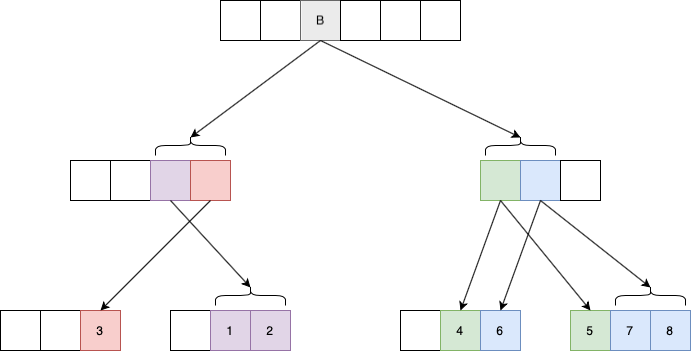
\includegraphics[width=5.5in]{pics/tree}
  \caption{Order of operations in b. Operations in the leaves are ordered with numerical order shown in the drawing.}
\end{figure}

Now we define the ordering of operations stored in each node. In the non-root nodes we only need to order operations of a type among themselves. Processes are numbered from 1 to $p$ and leaves of the tree are assigned from left to right. We will show in Lemma \ref{blockSize} that there is at most one operation from each process in a given block.
\begin{definition} [Ordering of operations inside the nodes] \label{ordering}
\end{definition}
\begin{itemize}
  \item $E(n,b)$ is the sequence of enqueue operations in $ops(n\nf{.blocks[}b\nf{]})$ defined recursively as follows. $E(leaf,b)$ is the single enqueue operation in $ops(leaf\nf{.blocks[}b\nf{]})$ or an empty sequence if $leaf\nf{.blocks[}b\nf{]}$ represents a dequeue operation. If $n$ is an internal node, then
\begin{align*} 
E(n,b) =&  E(n\nf{.left},n\nf{.blocks[}b-1\nf{].end\sub{left}}+1)\cdots E(n\nf{.left},n\nf{.blocks[}b\nf{].end\sub{left}})\cdot \\ 
&E(n\nf{.right},n\nf{.blocks[}b-1\nf{].end\sub{right}}+1)\cdots E(n\nf{.right},n\nf{.blocks[}b\nf{].end\sub{right}}).
\end{align*}
  \item $E_i(n,b)$ is the $i$th enqueue in $E(n,b)$.
\item The order of the enqueue operations in the node $n$ is $E(n)=E(n,1)\cdot E(n,2)\cdot E(n,3)\cdots$
\item $E_i(n)$ is the $i$th enqueue in $E(n)$.
  \item $D(n,b)$ is the sequence of dequeue operations in $ops(n\nf{.blocks[}b\nf{]})$ defined recursively as follows. $D(leaf,b)$ is the single dequeue operation in $ops(leaf\nf{.blocks[}b\nf{]})$ or an empty sequence if $leaf\nf{.blocks[}b\nf{]}$ represents an enqueue operation. If $n$ is an internal node, then
\begin{align*} 
D(n,b) =&  D(n\nf{.left},n\nf{.blocks[}b-1\nf{].end\sub{left}}+1)\cdots D(n\nf{.left}, n\nf{.blocks[}b\nf{].end\sub{left}})\cdot \\ 
&D(n\nf{.right},n\nf{.blocks[}b-1\nf{].end\sub{right}}+1)\cdots D(n\nf{.right},n\nf{.blocks[}b\nf{].end\sub{right}}).
\end{align*}
    \item $D_i(n,b)$ is the $i$th enqueue in $D(n,b)$.
\item The order of the dequeue operations in the node $n$ is $D(n)=D(n,1)\cdot D(n,2)\cdot D(n,3)...$
\item $D_i(n)$ is the $i$th dequeue in $D(n)$.
\end{itemize}


\begin{definition}[Linearization] \label{def::lin}
 $$L=E(root,1)\cdot D(root,1)\cdot E(root,2)\cdot D(root,2)\cdot E(root,3)\cdot D(root,3)\cdots$$
\end{definition}
\pagebreak

\subsection{Propagating Operations to the Root}
In this section we explain why two \nf{Refresh}es are enough to propagate a nodes operations to its parent.

\begin{definition}
Let $t^{op}$ be the time $op$ is invoked and $^{op}t$ be the time $op$ terminates.
  Let $t_{l}$ be the time immediately before executing Line $l$ and $_{l}t$ be the time immediately after executing Line $l$. Let $^{op}_{l}t$ is the time immediately before running Line $l$ of operation $op$ and   $t_{l}^{op}$ is the immediate time after running Line $l$ of operation $op$. In the text $v_l$ is the value of variable \nf{v} immediately after line $l$ for the process we are talking about and $v_t$ is the value of variable \nf{v} at time $t$.
\end{definition} 

\begin{definition} [Successful Refresh]
  An instance of \nf{Refresh()} is \it{successful} if its \nf{CAS} in Line \ref{cas} returns \nf{true}. If a successful instance of \nf{Refresh()} terminates, we say it is \it{complete.}
\end{definition}

In the next two results we show for every successful \nf{Refresh()}, all the operations established  in the children before the \nf{Refresh} are established in the parent after the \nf{Refresh}'s succesful \nf{CAS} at Line \ref{cas}.

\begin{lemma} \label{lem::trueRefresh}
If $R$ is a successful instance of \nf{$n$.Refresh()}, then we have $EST_{n\nf{.left}}^{t^R} \; \cup \; EST_{n\nf{.right}}^{t^R} \subseteq ops(n.blocks_{\ref{cas}})$.
\end{lemma}
\begin{proof}

We show 
\begin{align*}
EST_{n\nf{.left}}^{t^R}&= ops(n\nf{.left.blocks[0..n.left.head$_{309}-1$]}) \\
&\subseteq ops(n.blocks_{\ref{cas}}) = ops(n\nf{.blocks[0..}n.head_{\ref{cas}}\nf{]}).
\end{align*}

Line \ref{cas} stores a block \nf{new} in $n$ that has $\nf{end\sub{left}}=n.left.head_{\ref{lastLine}}-1$. Therefore by Definition \ref{def::subblock}, after the successful \nf{CAS} in Line \ref{cas} we know all blocks in \nf{$n$.left.blocks[$1\cdots n.left.head_{\ref{lastLine}}-1$]} are subblocks of \nf{n.blocks[$1\cdots n.head_{\ref{readHead}}$]}. Because of Lemma \ref{nonDecreasingHead} we have $n.left.head_{309}-1<n.left.head_{\ref{lastLine}}-1$ and $n.head_{\ref{readHead}}<n.head_{\ref{cas}}$. From Observation \ref{lem::blocksOrder} the claim follows.  The proof for the right child is the same.
\end{proof}

\begin{figure}[hbt]
  \center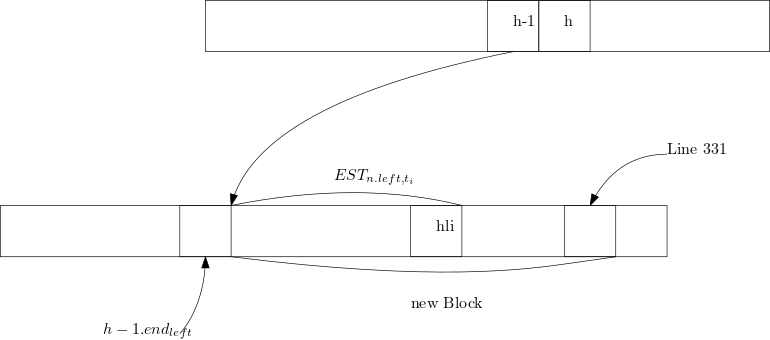
\includegraphics[width=5in]{pics/trueRefresh}
  \caption{TODO :: Is this picture good or should I remove it? New established operations of the left child are in the new block.(TO UPDATE)}
\end{figure}

\begin{corollary}\label{lem::prectrueRefresh}
If $R$ is a complete instance \nf{$n$.Refresh()}, then we have $EST_{n\nf{.left}}^{t^R} \; \cup \; EST_{n\nf{.right}}^{t^R} \subseteq EST_{n}^{^Rt}$.
\end{corollary}
\begin{proof}
The left hand side is the same as Lemma \ref{lem::trueRefresh}, so it is sufficient to show when \nf{R} terminates the established blocks in $n$ are a superset of $n$\nf{.blocks} after Line \ref{cas}.    Because of Lemma \ref{lem::headInc}  we are sure that $n$\nf{.head} is incremented after line \ref{incrementHead}. So the block \nf{new} appended to \nf{n} at Line \ref{cas} is established at $^Rt$. 
\end{proof}

\pagebreak

In the next lemma we show that if two consecutive instances of \nf{Refresh()} by the same process on node $n$ fail, then the established blocks in the children of $n$ before the first \nf{Refresh()} are guaranteed to be in $n$ after the second \nf{Refresh()}.

\begin{lemma} \label{doubleRefresh}
  Consider two consecutive terminating instances $R_1$, $R_2$ of \nf{Refresh()} on internal node $n$ by process $p$. If neither $R_1$ nor $R_2$ is a successful \nf{Refresh()}, then we have $EST_{n\nf{.left}}^{t^R{_1}} \; \cup \; EST_{n\nf{.right}}^{t^R{_1}} \subseteq EST_{n}^{^R{_2}t}$.
\end{lemma}
\begin{proof}
Let $R_1$ read $i$ from $n\nf{.head}$ at Line \ref{readHead}. Note that by Lemma \ref{lem::headInc} $R_1$ and $R_2$ both cannot read the same value $i$. By Observation \ref{nonDecreasingHead} $R_2$ reads larger value of $n$\nf{.head} than $R_1$.

Consider the case where $R_1$ reads $i$ and $R_2$ reads $i+1$ from Line \ref{readHead}. As $R_2$'s \nf{CAS} in Line \ref{cas} returns \nf{false}, there is another successful instance $R_2^\prime$ of \nf{n.Refresh()} that has done \nf{CAS} successfully into \nf{n.blocks[i+1]} before $R_2$ tries to \nf{CAS}. $R_2^\prime$ creates its block \nf{new} after reading the value $i+1$ from $n$\nf{.head} (Line \ref{readHead}) and $R_1$ reads the value $i$ from $n$\nf{.head}. By Observation \ref{nonDecreasingHead} we have $^{R_1}t<t^{R_1}_{\ref{readHead}}< t^{R2^\prime}_{\ref{readHead}}$ (see Figure \ref{fig::doubleRefresh}). By Lemma \ref{lem::prectrueRefresh} we have 
$EST^{n.\nf{left}}_{^{R_2^\prime}_{\ref{readHead}}t} \cup EST^{n.\nf{right}}_{^{R_2^\prime}_{\ref{readHead}}t} \subseteq ops(n.\nf{blocks}_{t_{\ref{cas}}^{R_2^\prime}})$. Also by Lemma \ref{lem::headInc} on $R_2$ the value  of \nf{n.head} is more than $i+1$ after $R_2$ terminates, so the block appended by $R_2^\prime$ to \nf{n} is established by the time $R_2$ terminates. To summarize, $^{R_1}t$ is before $R_2^\prime$'s read of \nf{n.head} ($t_{\ref{readHead}}^{R_2^\prime}$) and $R_2^\prime$'s successful \nf{CAS} ($t^{R2^\prime}_{\ref{cas}}$) is before $R_2$'s termination ($t^{R_2}$), so by Observation \ref{lem::blocksOrder} $ops(EST_{n.\nf{left}, t^{R_1}}) \cup ops(EST_{n.\nf{right}, t^{R_1}}) \subseteq ops(n.\nf{blocks}_{t^{R_2}})$

   If $R_2$ reads some value greater than $i+1$ in Line \ref{readHead} it means $n\nf{.head}$ has been incremented  more than two times since $_{\ref{readHead}}^{R_1}t$. By Lemma \ref{lem::headPosition}, when $n.$\nf{head} is incremented from $i+1$ to $i+2$, $n\nf{.blocks[i+1]}$ is non-null. Let $R_3$ be the \nf{Refresh()} on $n$ that has put the block in $n\nf{.blocks[}i+1\nf{]}$. $R_3$ read $n\nf{.head}=i+1$ at Line \ref{readHead} and has put its block in $n\nf{.blocks[}i+1\nf{]}$ before $R_2$'s read of $n.$\nf{head} at Line \ref{readHead}. So we have $t^{R_1}<_{\ref{readHead}}^{R_3}t<_{\ref{cas}}^{R_3}t<t^{R_2}_{\ref{readHead}}<^R_{2}t$. From Observation \ref{lem::blocksOrder} on the operations before and after $R_3$'s \nf{CAS} and Lemma \ref{lem::trueRefresh} on $R_3$ the claim holds.
\end{proof}

\begin{figure}[hbt]
  \center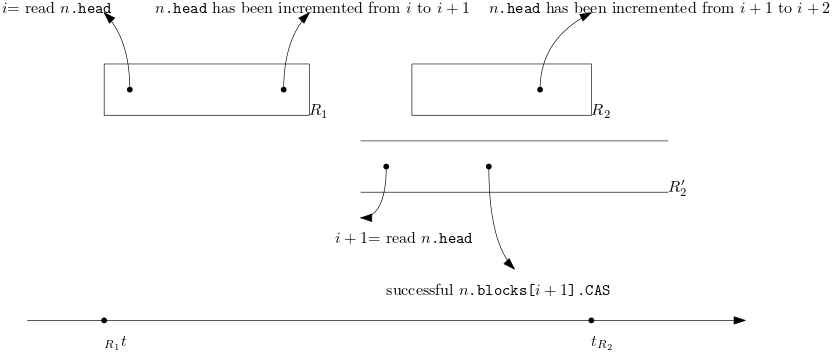
\includegraphics[width=6in]{pics/compactdouble.png}
  \caption{\label{fig::doubleRefresh}$_{R_1}t<$ $t_{\ref{readHead}}^{R_1}$ $<$ incrementing \nf{n.head} from $i$ to $i+1$ $<$ $t_{\ref{readHead}}^{R_2^\prime}$ $<$ $t_{\ref{cas}}^{R_2^\prime}$ $<$ incrementing \nf{n.head} from $i+1$ to $i+2$ $<t_{R_2}$} 
\end{figure}

\begin{corollary} \label{lem::propagateStep}
  \nf{ops(EST\sub{n.left, \sub{\ref{firstRefresh}}t})} $\cup$ \nf{ops(EST\sub{n.right, \sub{\ref{firstRefresh}}t})} $\subseteq$ \nf{ops(EST\sub{n, t\sub{\ref{secondRefresh}})}}
\end{corollary}
\begin{proof}
  If the first \nf{Refresh()} in line \ref{firstRefresh} returns \nf{true} then by Lemma \ref{lem::prectrueRefresh} the claim holds. If the first \nf{Refresh()} failed and the second \nf{Refresh()} succeeded the claim still holds by Lemma \ref{lem::prectrueRefresh}. Otherwise both failed and the claim is satisfied by Lemma \ref{doubleRefresh}.
\end{proof}

Now we show that after \nf{Append($b$)} on a leaf finishes, $b$ will be established in \nf{root}.

\begin{corollary}\label{lem::append}
For $A=\nf{Append(}b\nf{)}$ we have ${ops(b)} \subseteq ops(EST_{\nf{n}, t^A})$ where $n\in\{\text{nodes in the path from the leaf to the root}\}$.
\end{corollary}
\begin{proof}
$A$ adds $b$ to the assigned leaf of the process, establishes it at Line \ref{appendEnd} and then calls \nf{Propagate()} on the parent of the leaf where it appended $b$. For every node $n$, $n.$\nf{Propagate()} appends $b$ to $n$, establishes it by Corollary \ref{lem::propagateStep} and then calls $n.$\nf{parent.Propagate()} utill $n$ is \nf{root}.
\end{proof}

\begin{corollary}\label{lem::appendExactlyOnce}
 After \nf{Append($b$)} finishes, $b$ is in the nodes the path from the leaf to the root for exactly one time.
\end{corollary}
\begin{proof}
By the previous corollary and Lemma \ref{lem::appendExactlyOnce} there is exactly one block in each node containing $b$.
\end{proof}

\pagebreak

\subsection{Correctness of GetEnqueue}

Now we prove some claims about the size and operations of a block. These lemmas will be used for analysis and correctness of \nf{GetEnqueue()}.

\begin{lemma}\label{blockSize}
Each block contains at most one operation of each process.
\end{lemma}
\begin{proof}
To derive a contradiction, assume there are two operations $op_1$ and $op_2$ of process $p$ in block $b$ in node $n$. Without loss of generality $op_1$ is invoked earlier than $op_2$. Process $p$ cannot invoke more than one operations concurrently, so $op_1$ has to be finished before $op_2$ begins. By Corollary \ref{lem::appendExactlyOnce} before $op_2$ calls \nf{Append()}, $op_1$ exists in every node of the tree on the path from $p$'s leaf to the root. This means there is some block $b^\prime$ before $b$ in $n$ containing $op_1$. The Existence of $op_1$ in $b$ and $b^\prime$ contradicts Lemma \ref{lem::noDuplicates}.
\end{proof}

\begin{lemma}\label{subBlocksBound}
Each block has at most $p$ direct subblocks.
\end{lemma}
\begin{proof}
The claim follows directly from Lemma \ref{blockSize} and the observation that each block appended to an initial node contains at least one operation, due to the test on Line~\ref{addOP}. We can also see the blocks in the leaves have exactly one operation in the \nf{Enqueue()} and \nf{Dequeue()} routines.
\end{proof}

\nf{DSearch($e$, $end$)} returns \nf{<$b$, $i$>} so that $i$th \nf{Enqueue} in $b$th block of root is $e$th \nf{Enqueue} in entire sequence stored in the root. 
\begin{lemma}[\nf{DSearch} Correctness]\label{dsearch}
If $\nf{root.blocks[$end$]}\neq \nf{null}$ and $1\leq e \leq \nf{root.blocks[$end$].sum\sub{enq}}$, \nf{DSearch($e$, $end$)} returns \nf{<$b$, $i$>} such that $E_i(root,b)= E_e(root)$.
\end{lemma}
\begin{proof}
\nf{DSearch} performs a doubling search from \nf{root.blocks[end]} to \nf{root.blocks[0]} to find $E_e(root)$. From Lines \ref{setSumEnqLeft}, \ref{setSumEnqRight} we know \nf{sum\sub{enq-left}}, \nf{sum\sub{enq-right}} fields of \nf{blocks} in each node are sorted in non-decreasing order. Since $\nf{sum\sub{enq}}=\nf{sum\sub{enq-left}}+ \nf{sum\sub{enq-right}}$, $\nf{sum\sub{enq}}$ values of \nf{root.block[$0\cdot\cdot end$]} is  also non-decreasing. Furthermore, since $\nf{root.blocks[$0$].sum\sub{enq}}=0$ and $\nf{root.blocks[$end$].sum\sub{enq}} \geq e$, there is a $b$ such that $\nf{root.blocks[$b$].sum\sub{enq}} \geq e$ and $\nf{root.blocks[b-1].sum\sub{enq}} < e$. Block \nf{root.blocks[$b$]} contains $E_i(root,b)$. The doubling search on Lines \ref{dsearchStart}--\ref{dsearchEnd} doubles its search range in Line \ref{doubling} and will eventually reach \nf{start} such that $\nf{root.blocks[start].sum\sub{enq}}\leq e \leq\nf{root.blocks[end].sum\sub{enq}}$. In Line \ref{dsearchBinarySearch} Binary Search finds $b$ in the range mentioned. Finally $i$, is computed from the definition of \nf{sum\sub{enq}}.
\end{proof}


\begin{lemma}[\nf{GetEnqueue} correctness] \label{get}
If $1\leq i \leq \nf{$n$.blocks[$b$].num\sub{enq}}$ then \nf{$n$.GetEnqueue($b$, $i$)} returns $E_i(n,b)$\nf{.element}.
\end{lemma}
\begin{proof}
We are going to prove this lemma by induction on the height of node \nf{n}. For the base case, suppose $n$ is a leaf. Leaf blocks each contain exactly one operation, so only \nf{$n$.GetEnqueue(b,1)} can be called when $n$ is a leaf. Line \ref{getBaseCase} of \nf{$n$.GetEnqueue($b$, $1$)} returns the \nf{element} of the \nf{Enqueue} operation stored in the $b$th block of leaf ${n}$.

For the induction step we prove if \nf{$n$.child.GetEnqueue($sb$, i)} returns $E_i(n.child, sb)$ then \nf{$n$.GetEnqueue($b$, $i$)} returns $E_i(n,b)$.  From Definition \ref{ordering} of $E(n,b)$, operations from the left subblocks come before the operations from the right subblocks in a block (see Figure \ref{figGet}). \nf{num\sub{enq-left}} field  in \nf{$n$.blocks[$b$]} is the number of \nf{Enqueue()} operations from the blocks's subblocks in the left child of \nf{n}. So the $i$th enqueue operation is propagated from the right child if and only if $i$ is greater than \nf{$b$.num\sub{enq-left}}. Line \ref{leftOrRight} decides whether the \nf{i}th enqueue in  $b$th block  of internal node \nf{n} is in the  left child or right child subblocks of \nf{n.blocks[b]}. By Definitions \ref{def::ops}, \ref{def::subblock} to find an operation in subblocks of \nf{$n$.blocks[$i$]} we need to search in the range
\begin{align*}
&\texttt{$n$.left.blocks[$n$.blocks[$i$-1].end\textsubscript{left}+1..$n$.blocks[$i$].end\textsubscript{left}]}  \cup \\
&\texttt{$n$.right.blocks[$n$.blocks[$i$-1].end\textsubscript{right}+1..$n$.blocks[$i$].end\textsubscript{right}]}.
 \end{align*}
First we consider the case where the \nf{Enqueue} we are looking is in the left child. There are $eb=n.\nf{blocks[}b-1\nf{].sum\sub{enq-left}}$ enqueues in the blocks before the left subblocks of $n$\nf{.blocks[$b$]}, so $E_i(n,b)$ is $E_{i+eb}(n.left)$ which is $E_{i^\prime}(n.left,b^\prime)$ for some $b^\prime$ and $i^\prime$. We can compute $b^\prime$ and then search for the $i+eb$th enqueue in \tt{n.left}, where $i^\prime$ is \tt{i+eb-n.left.blocks[}$b^\prime-1$\tt{].sum\sub{enq}}. The parameters in Line \ref{leftChildGet} are for searching $E_{i+eb}(n.left)$ in \nf{n.left.block} in the range of left subblocks of $n$\nf{.blocks[}$b$\nf{]}, so this \nf{BinarySearch} returns the index of the subblock containing $E_i(n,b)$.

Otherwise, the enqueue we are looking for is in the right child. Because \nf{Enqueue}s from the left subblocks are ordered before the \nf{Enqueue}s from the right subblocks, there are \nf{n.blocks[b].num\sub{enq-left}} enqueues ahead of $E_i(n,b)$ from the left child. So we need to search for $i-n\nf{.blocks[}b\nf{].num\sub{enq-left}}+ n\nf{.blocks[}b-1\nf{].sum\sub{enq-right}}$ (Line \ref{rightChildGet}). Other parameters for the right child are chosen similarly to the left child. 

So, in both cases the direct subblock containing $E_i(n,b)$ is computed in Line \ref{leftChildGet} or \ref{rightChildGet}.
 Finally, \nf{n.child.GetEnqueue(subblock, i)} is invoked on the subblock containing $E_i(n,b)$ and it returns $E_i(n,b)$ by the hypothesis of the induction.
\end{proof}

\begin{figure}[hbt]  
  \center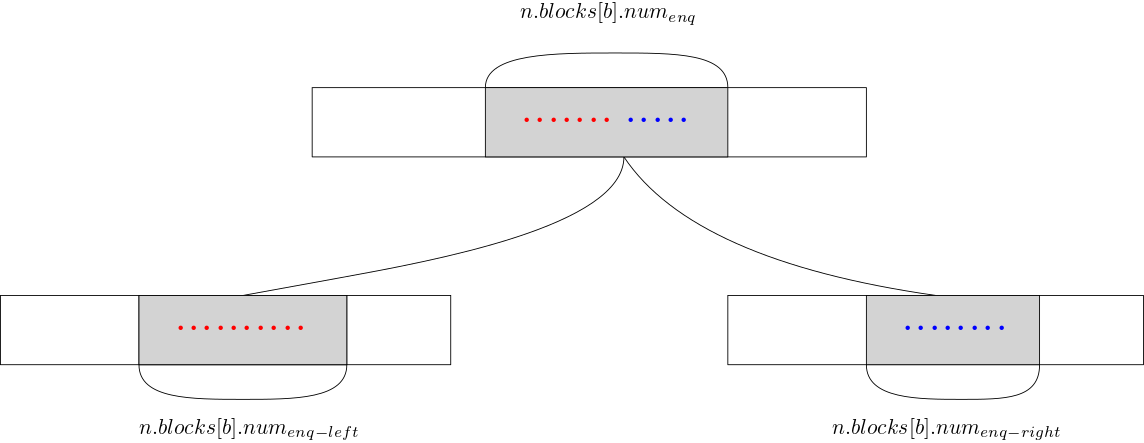
\includegraphics[width=6in]{pics/blockSumEnq.png}
  
  \caption{The number and ordering of the enqueue operations propagated from the left and the right child to \nf{n.blocks[b]}. Enqueue operations from the left subblocks (colored red), are ordered before the enqueue operations from the right child (colored blue).
  }\label{figGet}
\end{figure}

\clearpage

\subsection{Correctness of IndexDequeue}
\begin{definition}\label{orderRefresh} If \nf{Refresh} instance $R_1$ does its \nf{CAS} at Line \ref{cas} earlier than \nf{Refresh} instance $R_2$ we say $R_1$ has \it{happened before} $R_2$.
\end{definition}

\begin{observation} \label{setSupBeforeIncHead}
After \nf{$n$.blocks[$i$].CAS(null, $b$)} succeeds, \nf{$n$.head} cannot increase from ${i}$ to ${i+1}$ unless \nf{$b$.super} is set.
\end{observation}
\begin{proof}
From the Observation \ref{nonDecreasingHead} we know the only change to \nf{n.head} is on Line \ref{incrementHead} which is incrementing. Before an instance of \nf{Advance()} increments \nf{n.head} on Line \ref{incrementHead}, Line \ref{setSuper1} ensures that \nf{n.blocks[head].super} was set at Line \ref{setSuper1}.
\end{proof}

\begin{corollary}
  If \nf{n.blocks[i].super} is \nf{null}, then $\nf{n.head}<\nf{i}$ and \nf{n.blocks[i+1]} is \nf{null}.
\end{corollary}
\begin{proof}
By Lemma \ref{lem::headPosition} and Observation \ref{setSupBeforeIncHead}.
\end{proof}
Now let us talk about how the \nf{$p$.Refresh}es that took place after the putting $b$ into \nf{n}, will help to set \nf{b.super} and propagate $b$.

\begin{lemma}
  If $b$ is a direct subblock of \nf{$n$.parent.blocks[$i$]} then $\nf{$b$.super}\leq i$.
\end{lemma}
\begin{proof}
Instance $R_p$ of $n$\nf{.parent.Refresh()} contains block $b$, if it reads \nf{$n$.head} greater than ${h}$, the index of $b$ in $n$ (see Line \ref{lastLine}). For \nf{$n$.head} to be greater than ${h}$ it means \nf{$n$.head} is incremented in Line \ref{incrementHead} which means \nf{$b$.super} was already set in Line \ref{setSuper1} (see Observation \ref{setSupBeforeIncHead}). So if $R_p$ propagates $b$ it means \nf{$b$.super} was already set. The value written in \nf{b.super} has been read in Line \ref{readHead} or Line \ref{readParentHead} which both are before calling \nf{Advance} that sets \nf{$b$.super}. From Observation \ref{nonDecreasingHead} we know \nf{$n$.parent.head} is non-decreasing so $b\nf{.super}\leq\nf{i}$. The reader may wonder when the case $b\nf{.super}=\nf{i}$ happens, it happens when $\nf{$n$.parent.blocks[$b$.super]}=\nf{null}$ while $b$\nf{.super} is read and $R_p$ puts its created block into \nf{n.blocks[$b$\nf{.super}]}.
\end{proof}

\begin{lemma}
If $R_n=$\nf{Refresh()} puts $b$ in \nf{$n$.blocks[$h$]} at Line \ref{cas}, then the block created by one of the next two successful \nf{$n$.parent.Refresh}es according to the Definition \ref{orderRefresh} contains $b$ and \nf{$b$.super} is set before Line \ref{invokeCreateBlock} of the the second successful \nf{$n$.parent.Refresh()}.
\end{lemma}

\begin{proof}
It is sufficient to prove one of the two successful \nf{$n$.parent.Refresh()}es propagates $b$. If the first successful \nf{p.Refresh()} propagated $b$ then the claim is true. We prove if the first \nf{$n$.parent.Refresh()} did not propagate $b$, second \nf{$n$.parent.Refresh()} propagates $b$.

\nf{$b$.super} is set by some instance of \nf{Refresh()} on $n$ or \nf{$n$.parent} showed by $R^\prime$ and \nf{$n$.head} is incremented by some \nf{Refresh()} called $R^\prime\prime$. Let \nf{$n$.parent.head} value be $hp$ when $R^\prime$ reads it. From Lemma \ref{lem::headProgress} \nf{$n$.parent.head} could only increase from ${hp}$ to ${hp+1}$ if $\nf{$n$.parent.blocks[$hp$]}\neq\nf{null}$. In other words there should be a successful \nf{$n$.parent.Refresh()} for \nf{$n$.parent.head} to be increased. Let $R_p$ be \nf{$n$.parent.Refresh} that propagated $b$ to \nf{$n$.parent}. We claim there cannot be another successful \nf{$n$.parent.Refresh()} after $R^\prime$ reads \nf{$n$.parent.head} and before $R_p$ performs Line \ref{lastLine}.

\begin{figure}[hbt]  
  \center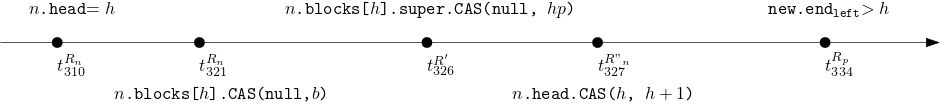
\includegraphics[width=5.5in,height=0.65in]{pics/timeLineSuper1.png}
  \caption{Time relations between \nf{R\sub{n},R\sub{p},R',R"}}
  \label{fig::timeLine1}
\end{figure}

Without loss of generality  assume $n$ is the left child of \nf{$n$.parent}. As we mentioned the first successful \nf{$n$.parent.Refresh()} after $t_{\ref{cas}}^{Rn}$ did not set \nf{$b$.super}. It might happen maybe because the value $h_{left}$ read for $n$\nf{.head} in Line \ref{readChildHead} is less than or equal to $i$ and $\nf{left.blocks[$h_{left}$]}=\nf{null}$, which means \nf{$n$.head} is advanced but $b$ is still not installed in \nf{$n$.blocks[$i$]} which means $R_n$ has not reached  the Line \ref{cas}.
  
Let the first successful \nf{$n$.parent.Refresh()} be $R_{p1}$ and the second next successful \nf{$n$.parent.Refresh()} be $R_{p2}$. If $R_{p1}$ reads $x$ in Line \ref{readHead}, then $R_{p2}$ has to read ${x+1}$ in Line \ref{readHead} (induced from \ref{lem::headProgress}, \ref{nonDecreasingHead}). See the timeline in Figure \ref{fig::timeLine2} for two consecutive successful \nf{Refresh()} instances $R_{p1}$,$R_{p2}$ on \nf{$n$.parent}.

\begin{figure}[hbt]  
  \center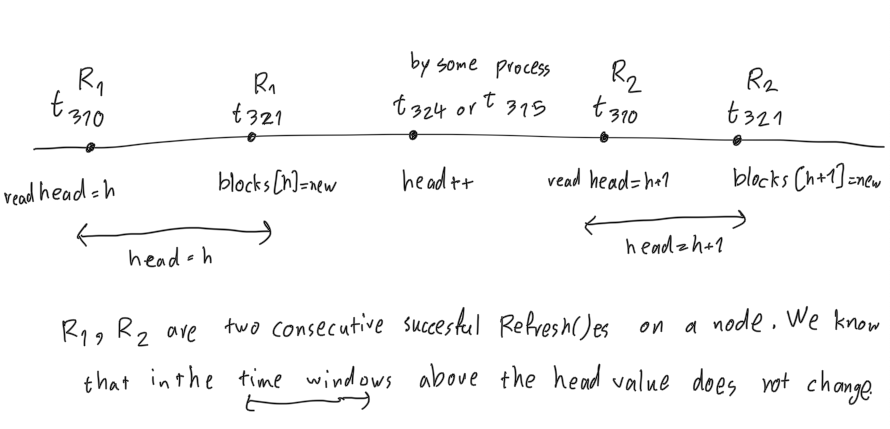
\includegraphics[width=6in,height=1.25in]{pics/timeLineSuper2.png}
  \caption{$R_{p2}$ reads \nf{$n$.parent.head} after $t_{320}^{R_{p1}}$, which is after $t_{320}^{Rn}$. $R_{p2}$ has to help increment \nf{$n$.head} and set $b$\nf{.super}.}
  \label{fig::timeLine2}
\end{figure}

$$t_{\ref{cas}}^{R_n}<t_{\ref{cas}}^{R_p}<t_{\ref{cas}}^{R_p'}<t_{314}^{R_p'}$$
$t_{\ref{cas}}^{R_n}<t_{\ref{cas}}$ because $R_p$ is the first successful $p.Refresh()$ after $R_n$. $t_{\ref{cas}}^{R_p}<t_{\ref{cas}}^{R_p'}$ because of the time windows between two consecutive successful \nf{Refresh()} instances on a node. $t_{\ref{cas}}^{R_p'}<t_{314}^{R_p'}$ because it is sequential in the code. The second Refresh on \nf{p} contains $b$ and reads $\nf{n.head}>\nf{i}$.

So \nf{$b$.super} has set by some process before the second next successful \nf{$n$.parent.Refresh()} on Line \ref{setSuper1}. Since $i$ is read in the Line \ref{readHead} then the \nf{CreateBlock()} in Line \ref{invokeCreateBlock} is going to read  some value for \nf{left.head} greater than ${h}$ and propagates $b$ to \nf{$n$.parent}. So if $b$ was not propagated already we are sure the second next successful \nf{$n$.parent.Refresh()} propagates $b$.
\end{proof}

\begin{corollary} \label{superRelation}
If \nf{$n$.blocks[$b$]} is propagated to $n$\nf{.parent}, then \nf{$n$.blocks[$b$].super} is equal to or one less than the index of the superblock of \nf{$n$.blocks[$b$]}.
\end{corollary}

Now using Corollary \ref{superRelation} on each step of the \nf{IndexDequeue} we prove its correctness.

\begin{lemma}[\nf{IndexDequeue} correctness]
 If $1\leq i \leq\nf{$n$.blocks[$b$].num\sub{deq}}$ then \nf{$n$.IndexDequeue($b$,$i$)} returns the rank in $D(root)$ of $D_i(n,b)$.
\end{lemma}
\begin{proof}
We will prove this by induction on the distance of $n$ from the \nf{root}. The base case where $n$ is \nf{root} is trivial (Line \ref{indexBaseCase}).
For the non-root nodes \nf{$n$.IndexDequeue($b$, $i$)} computes the superblock of the $b$th block of $n$ in Line \ref{computeSuper} by Corollary \ref{superRelation}. So preconditions of the invocation of \nf{BinarySearch} is satisfied. After that the order of $D_i(n,b)$ in $D(n.parent, superblock)$ is computed in Lines \ref{computeISuperStart}--\ref{computeISuperEnd}. By Lemma \ref{blockSize} in each block there is at most one \nf{Dequeue} from each process and by Definition \ref{ordering} \nf{Dequeue}s in a block are ordered based on the order of its subblocks  from left to right. Then if $D_i(n,b)$ was propagated from the right child, the number of dequeues in the subblocks from the left child is considered to be ahead of the computed index (Line \ref{considerRight}). Finally \nf{IndexDequeue} is called on \nf{$n$.parent} recursively and it returns the response from induction hypothesis. 
\end{proof}

\pagebreak
\subsection{Linearizability}
We now prove the two properties needed for linearizability.

\begin{lemma} \label{linearSat}
$L$ is a legal linearization ordering.
\end{lemma}
\begin{proof}
A linearization for an execution is legal if, $op_{1}$ terminates before $op_{2}$ starts in execution then $op_{1}$ is before $op_{2}$ in the linearization. If $op_{1}$ terminates before $op_{2}$ starts,  $op_{1}$\nf{.Append()} has terminated before $op_{2}$\nf{.Append()} started. From Lemma \ref{lem::append} $op_{1}$ is in \nf{root.blocks} before $op_{2}$ starts to propagate. By definition of $L$, $op_{1}$ is linearized before $op_{2}$.
\end{proof}
Once some operations are aggregated in one block, they will get propagated up to the root together and they can be linearized in any order among themselves. The way we have chosen to order the operations in a block makes \nf{GetEnqueue} and \nf{FindResponse} efficient.

\begin{definition}\label{defNullDeq}
If a \nf{Dequeue} operation returns null it is called a \it{null dequeue}, otherwise it is called \it{non-null dequeue}.
\end{definition}

\begin{definition}
   Assume the operations in \nf{root.blocks} are applied sequentially on an empty queue in the order of $L$.  ${Resp(d)=e}$\nf{.element} if the element of \nf{Enqueue} $e$ is the response to \nf{Dequeue} $d$. Otherwise if ${d}$ is a null dequeue then ${Resp(d)=\nf{null}}$. 
\end{definition}

\begin{observation}\label{enqBeforeDeq}
By Definition \ref{ordering} enqueue operations come before dequeue operations in a block.  
\end{observation}

In the next lemma we show that the \nf{size} field in each \nf{root block} is computed correctly.
\begin{lemma}\label{sizeCorrectness}
  \nf{root.blocks[$b$].\size}is the \size of the queue if the operations in \nf{root.blocks[$0\cdots b$]} are applied in the order of~$L$.  
\end{lemma}
\begin{proof}
We prove the claim by induction on $b$. The base case when ${b=0}$ is trivial since the queue is initially empty and $\nf{root.blocks[}0\nf{].size}=0$. We are going to show the correctness when $b=i$ assuming  correctness when $b=i-1$. By Observation \ref{enqBeforeDeq} if there are more than $\nf{root.blocks[}i-1\nf{].size}+\nf{root.blocks[}i\nf{].sum\sub{enq}}$ dequeue operations in \nf{root.blocks[$i$]} then the queue would become empty after \nf{root.blocks[$i$]}. Otherwise the size of the queue after the $b$th block in the root is $\nf{root.blocks[}b-1\nf{].size}+ \nf{root.blocks[}b\nf{].sum\sub{enq}}- \nf{root.blocks[}b\nf{].sum\sub{deq}}$. In both cases, this is same as the assignment on Line \ref{computeLength}.
\end{proof}

The next lemma is useful to compute the number of non-null dequeues.
\begin{lemma} \label{numberOfNND}
If operations in the root are applied with the order of $L$, the number of non-null dequeues in $\nf{root.blocks[}0\cdots b\nf{]}$ is \nf{root.blocks[$b$].sum\sub{enq} $-$ root.blocks[$b$].size}.
\end{lemma}
\begin{proof}
There are \nf{root.blocks[$b$]}\nf{.sum\sub{enq}} enqueue operations in $\nf{root.blocks[}0\cdots b\nf{]}$. The size of the queue after doing $\nf{root.blocks[}0\cdots b\nf{]}$ in order $L$ is 
$\#\it{enqueues}$ in $\nf{root.blocks[}0\cdots b\nf{]}$ $-$ $\#\it{non-null dequeues}$ in $\nf{root.blocks[}0\cdots b\nf{]}$. By the correctness of the \nf{size} field from Lemma \ref{sizeCorrectness}, $\it{\#non-null dequeues}$ is \nf{root.blocks[$b$]}\nf{.sum\sub{enq}} $-$ \nf{root.blocks[$b$]}\nf{.size}. 
\end{proof}

\begin{corollary}\label{numNullDeqBlock}
  If operations in the root are applied with the order of $L$, the number of non-null dequeues in $\nf{root.blocks[}b\nf{]}$ is \nf{root.blocks[$b$].num\sub{enq} $-$ root.blocks[$b$].\size $+$ root.blocks[$b-1$].size}.
\end{corollary}

\begin{lemma}\label{nullReturn}
\nf{R(D\sub{root,b,i})} is \nf{null} iff \nf{root.blocks[$b-1$].\size $+$ root.blocks[$b$].num\sub{enq}$- i$ $<0$}.
\end{lemma}
\begin{proof}
From Corollary \ref{numNullDeqBlock} and Observation \ref{enqBeforeDeq}.
\end{proof}

\begin{lemma}\label{computeHead}
\nf{FindResponse($b$, $i$)} returns $Resp(D_i(root,b))$.
\end{lemma}
\begin{proof}
$D_i(root,b)$ is $D_{\nf{root.blocks[}b-1\nf{].sum\sub{deq}}+i}(root)$ by Definition \ref{ordering} and Lemma \ref{lem::sumDeq}. $D_i(root,b)$ returns \nf{null} at Line \ref{returnNull} if $\nf{root.blocks[}b-1\nf{].size}+ \nf{root.blocks[}b\nf{].num\sub{enq}}- i <0$ and $Resp(D_i(root,b))=\nf{null}$ in this case by Lemma \ref{nullReturn}. Otherwise if $D_i(root,b)$ is $e$th non-null dequeue in $L$ it should return $e$th enqueued value. By Lemma \ref{numberOfNND} there are \nf{root.blocks[$b-1$].sum\sub{enq} $-$ root.blocks[$b-1$].\size} non-null dequeue operations in $\nf{root.blocks[}0\cdots b-1\nf{]}$. The dequeues in the \nf{root.blocks[$b$]} before $D_i(root,b)$ are non-null dequeues. So $Resp(D_i(root,b))$ is the \nf{element} field of $e$th non-null dequeue when $e=i - root.blocks[b-1].size + root.blocks[b-1].sum\sub{deq}$ (Line \ref{computeE}). See Figure \ref{computeResponseDetail}.

After computing \nf{e} at Line \ref{computeE}, the code finds \nf{$b$,$i$} such that $E_i(root,b)=E_e(root)$ using \nf{DSearch} and then finds its \nf{element} using \nf{GetEnqueue} (Line \ref{findAnswer}).
\end{proof}

\begin{figure}[hbt]  
  \center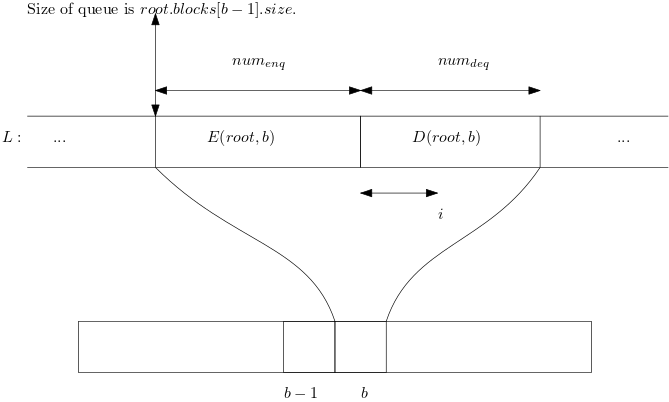
\includegraphics[width=4in, height=2.5in]{pics/computeResponseDetail.png}\caption{The position of $D_i(root,b)$.}
\label{computeResponseDetail}
\end{figure}

\begin{lemma}\label{linearCorrect}
The responses to operations in our algorithm would be the same as in the sequential execution in the order given by $L$.
\end{lemma}
\begin{proof}
Enqueue operations do not return any value. By \ref{computeHead} response of a dequeue in our algorithm is same as the response from the sequential execution of $L$.  
\end{proof}

\begin{theorem}[Main]
The queue implementation is linearizable.
\end{theorem}
\begin{proof}
From \ref{linearSat}, \ref{linearCorrect}.
\end{proof}

\paragraph{Remark} In fact our algorithm is strongly linearizable \cite{DBLP:conf/stoc/GolabHW11}. By Definition \ref{ordering} the linearization ordering of operations will not change as new operations come.
\pagebreak

\section{Analysis}
\begin{lemma}[Amortized time analysis]
\nf{Enqueue()} and \nf{Dequeue()}, each take $O(\log^2 p + \log q)$ steps in amortized analysis. Where $p$ is the number of processes and $q$ is the size of the queue at the time of invocation of operation.
\end{lemma}
\begin{proof}
\nf{Enqueue(x)} consists of creating a \nf{block(x)} and appending it to the tree. The first part takes constant time. To propagate \nf{x} to the root the algorithm tries two \nf{Refresh}es in each node of the path from the leaf to the root (Lines \ref{firstRefresh}, \ref{secondRefresh}). We can see from the code  that each \nf{Refresh} takes constant number of steps since creating a block is done in constant time and does $O(1)$ \nf{CAS}es. Since the height of the tree is $\Theta(\log p)$, \nf{Enqueue(x)} takes $O(\log p)$ steps.

A \nf{Dequeue()} creates a block with null value element, appends it to the tree, computes its order among enqueue operations, and returns the response. The first two part is similar to an \nf{Enqueue} operation. To compute the order of a \nf{dqueue} in $D(n)$ there are some constant steps and \nf{IndexDequeue()} is called. \nf{IndexDequeue} does a search with range $p$ in each level (Lemma \ref{superRange}) which takes $O(log^2 p)$ in the tree. In the \nf{FindResponse()} routine \nf{DSearch()} in the root takes $\Theta(\log$(\nf{root.blocks[b].\size+root.blocks[end].\size}) by Lemma \ref{dsearch}, which is $O(\log$ size of the queue when \nf{enqueue} is invoked$)+\log$ size of the queue when \nf{dequeue} is invoked$)$. Each search in \nf{GetEnqueue()} takes $O(\log p)$ since there are $\leq p$ subblocks in a block (Lemma \ref{subBlocksBound}), so \nf{GetEnqueue()} takes $O(\log^2 p)$ steps.

If we split \nf{DSearch} time cost between the corresponding \nf{Enqueue}, \nf{Dequeue}, in amortized we have \nf{Enqueue} takes $O(\log p +q)$ and \nf{Dequeue} takes $O(\log^2 p +q)$ steps.
\end{proof}

\begin{lemma}
An \nf{Enqueue()} or \nf{Dequeue()} operation, does at most $4\log p$ \nf{CAS} operations.
\end{lemma}
\begin{proof}
  In each height of the tree at most 2 times \nf{Refresh()} is invoked and  every \nf{Refresh()} has 2 \nf{CAS}es, one in Line \ref{cas} and one in Lines \ref{incrementHead1} or \ref{incrementHead2}.
\end{proof}

\begin{lemma}[\nf{DSearch} Analysis]\label{dsearchTime}
If the \nf{element} enqueued by $E_i(root,b)=E_e(root)$ is the response to some \nf{Dequeue()} operation in \nf{root.blocks[end]}, then \nf{DSearch($e$, $end$)} takes $O\big(\log ( \nf{root.blocks[$b$].size}+ \nf{root.blocks[$end$].size})\big )$ steps.
\end{lemma}
\begin{proof}
First we show $end - b -1\leq 2 \times \nf{root.blocks[$b-1$].size}+\nf{root.blocks[$end$].size}$. Suppose there were more than \nf{root.blocks[b].size} \nf{Dequeue}s in \nf{root.blocks[$b+1 \cdots end-1$]}. Then the element in the queue which is the response to the \nf{Dequeue()} would become dequeued at some point before \nf{root.blocks[$end$]}'s first \nf{Dequeue()}. Furthermore in the execution of queue operations in the linearization ordering, the size of the queue becomes \nf{root.blocks[$end$].size} after the operations of \nf{root.blocks[$end$]}. There can be at most \nf{root.blocks[$b$].size}  \nf{Dequeue}s in \nf{root.blocks[$b+1\cdots end-1$]}; otherwise all elements enqueued by \nf{root.blocks[$b$]} would be dequeued before \nf{root.blocks[$end$]}.  The final size of the queue after \nf{root.blocks[$1\cdots end$]} is \nf{root.blocks[$end$].size}. After an execution on a queue the $size$ of the queue is greater than or equal to $\#enqueues -\#dequeues$ in the execution.We know the number of dequeues in \nf{root.blocks[$b+1\cdots end-1$]} is less than \nf{root.blocks[$b$].size}, therefore there cannot be more than $\nf{root.blocks[$b$].size} + \nf{root.blocks[$end$].size}$ \nf{Enqueue}s in \nf{root.blocks[$b+1\cdots end-1$]}. Overall there can be at most $2 \times\nf{root.blocks[$b$].size}+ \nf{root.blocks[$end$].size}$ operations in \nf{root.blocks[$b+1\cdots end$]} and since from line \ref{addOP} we know that \nf{num} field of the every block in the tree is greater than 0, each block has at least one operation, there are at most $2 \times\nf{root.blocks[$b$].size}+ \nf{root.blocks[$end$].size}$ blocks in between \nf{root.blocks[$b$]} and \nf{root.blocks[$end$]}. So $end-b-1\leq 2 \times\nf{root.blocks[$b$].size}+\nf{root.blocks[$end$].size}$.

So the doubling search reaches \nf{start} such that the \nf{root.blocks[start].sum\sub{enq}} is less than $e$ in $O \big(\log(\nf{root.blocks[$b$].size}+\nf{root.blocks[$end$].size})\big)$ steps. See Figure \ref{fig::doubling}. After Line \ref{dsearchEnd}, the binary search that finds $b$ also takes $O\big(\log(\nf{root.blocks[$b$].size}+\nf{root.blocks[$end$].size})\big)$. Next, \nf{i} is computed via the definition of \nf{sum\sub{enq}} in constant time (Line \ref{DSearchComputei}). So the claim is proved.
\end{proof}
\begin{figure}[hbt]  
  \center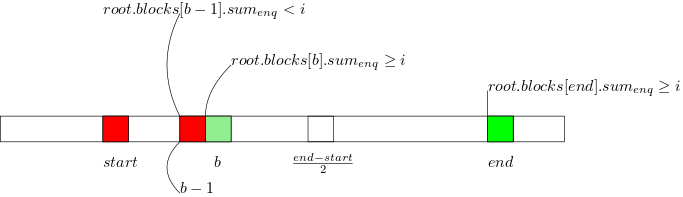
\includegraphics[width=6in]{pics/doubling.png}
  \caption{Distance relations between \nf{start}$,b,end$.}
  \label{fig::doubling}
\end{figure}

\pagebreak
\subsection{Garbage Collection or Getting rid of the infinite Arrays}

\pagebreak
\section{Using Queues to Implement Vectors}
Supporting Append, Read, Write in PolyLog time by modifying Get(Enq) Method. Create a Universal Construction Using our vector

\pagebreak
\section{Conclusion}
possible directions for work

Maybe Stacks

Characterize what datastructure can be used for this approach, we already know: queue, fetch \& Inc, Vectors

\section*{References}
\bibliography{main.bib} 
\bibliographystyle{plain}

\end{document}

